\documentclass[a4paper,12pt]{article}
\usepackage{standalone}
\usepackage[a4paper, top=0.8in, bottom=0.7in, left=0.8in, right=0.8in]{geometry}
\usepackage{amsmath}
\usepackage{hyperref}
\usepackage{amsfonts}
\usepackage{latexsym}
\usepackage{graphicx}
\usepackage{fancyhdr}
\usepackage{enumitem}
\usepackage{setspace}
\usepackage{tcolorbox}
\usepackage{tikz}
\usepackage{multicol}
\usepackage[defaultfam,tabular,lining]{montserrat} % Font settings for Montserrat
\usepackage{xcolor}  % To use colors

\hypersetup{
    colorlinks=true,   % Activate colored links
    linkcolor=blue,    % Link color for internal links
    urlcolor=blue,     % Link color for URLs
    filecolor=blue,    % Link color for file links
    menucolor=blue     % Link color for menus
}

\sloppy
\title{}
\date{}
\hyphenpenalty=10000
\exhyphenpenalty=10000
\setlength{\parindent}{0pt}
\pagestyle{fancy}
\setlength{\headheight}{27.11148pt}
\addtolength{\topmargin}{-15.11148pt}
% Define new commands for subject, assessment type, and Level
\newcommand{\standards}{CCSS} 
\newcommand{\subject}{Math} 
\newcommand{\doctype}{TWB}
\newcommand{\levelLetter}{D}


% Change these commands to update throughout the document


%Document Title Command
\newcommand{\doctitle}{\standards \ \subject  \ Curriculum \levelLetter \ \doctype }



\fancyhf{}
\fancyhead[L]{\textbf{\doctitle}}
\fancyhead[R]{
\includegraphics[width=0.8cm]{Round Logo.png}} % Placeholder for logo
\fancyfoot[C]{\footnotesize \textcopyright{} Study Smart Tutors}
\fancyfoot[R]{\thepage}  % Page number in bottom right corner
\fancyfoot[L]{\hyperlink{toc}{Back to Contents}} % Clickable link in bottom left to TOC



\begin{document}


% Title Page
\documentclass[12pt]{article}
\usepackage[a4paper, top=0.8in, bottom=0.7in, left=0.8in, right=0.8in]{geometry}
\usepackage{amsmath}
\usepackage{amsfonts}
\usepackage{latexsym}
\usepackage{graphicx}
\usepackage{tikz}
\usepackage{fancyhdr}
\usepackage{tcolorbox}
\usepackage{multicol}
\usepackage{tgadventor}
\renewcommand{\familydefault}{\sfdefault}
\usepackage{enumitem}
\usepackage{setspace}
\setlength{\parindent}{0pt}
\pagestyle{fancy}
\usepackage{needspace}


% Define a new command for the level letter
\newcommand{\levelLetter}{D}  % Change this letter to update throughout the document

%%%%%%%%%%%%%%%%%%%%%%%%%%%%%%%%%%%%%

\setlength{\headheight}{27.11148pt}
\addtolength{\topmargin}{-15.11148pt}

\fancyhf{}
%\fancyhead[L]{\textbf{5.NBT.A.1: Understand the Place Value System}}
\fancyhead[R]{
\includegraphics[width=0.8cm]{Round Logo.png}}
\fancyfoot[C]{\footnotesize © Study Smart Tutors}






\title{}
\date{}
\hyphenpenalty=10000
\exhyphenpenalty=10000

\begin{document}


%%%%%%%%%%%%%%%%%%%%%%%%%%%%%%%%%%%%%%%%%%%%%%%%%%%%%%%%%%%%%%%%%%%%


% INSTRUCTOR COVER PAGE BEGIN
% Skip header and footer on the first page
\thispagestyle{empty}

% Vertical centering
\vspace*{\fill}

\vspace*{3cm}

\begin{center}

    % Logo
    
\includegraphics[width=0.6\textwidth]{SST_Color_Logo.png} % Replace 'logo.png' with the path to your logo file
    
    \vspace{2cm} % Space between logo and title
    
    % Cycle Name

    
    % Assessment Title
    \Huge \textbf{Mathematics  Tutoring}\\
    [0.3cm]
     \vspace{1cm}
    \LARGE \textit{Curriculum \levelLetter}\\[1cm] 
   

    \Huge \textbf{INSTRUCTOR VERSION}
    
   
    
    \vfill % Push the footer to the bottom
    
\end{center}
\newpage
\thispagestyle{empty}
\vspace*{\fill}
\newpage

% INSTRUCTOR VERSION COVER PAGE COMPLETE




% *************************



\end{document}
 % Include the title page content here
\pagenumbering{gobble}
\hypertarget{toc}{}  % Mark the TOC as a hyperlink target
\tableofcontents
\newpage

% Restart page numbering from 1 after TOC
\pagenumbering{arabic}
\pagestyle{fancy}  % Re-enable fancy headers/footers

% Guided Lesson and Answer Key for 3.OA.A.1, 3.OA.A.3
\newpage
\section{3.OA.A.1, 3.OA.A.3 Guided Lesson (Instructor Version)}
\documentclass[12pt]{article}
\usepackage[a4paper, top=0.8in, bottom=0.7in, left=0.8in, right=0.8in]{geometry}
\usepackage{amsmath, amsfonts, latexsym, graphicx, fancyhdr, enumitem, setspace, tcolorbox, textcomp, xcolor}
\usepackage[defaultfam,tabular,lining]{montserrat} % Font settings for Montserrat

\setlength{\parindent}{0pt}
\pagestyle{fancy}

\setlength{\headheight}{27.11148pt}
\addtolength{\topmargin}{-15.11148pt}

\fancyhf{}
%\fancyhead[L]{\textbf{Standard(s): 3.OA.A.1, 3.OA.A.3}} % Example standards
\fancyhead[R]{
\includegraphics[width=0.8cm]{Round Logo.png}} % Placeholder for logo
\fancyfoot[C]{\footnotesize \textcopyright Study Smart Tutors}

\title{}
\date{}
\hyphenpenalty=10000
\exhyphenpenalty=10000

\begin{document}

\subsection*{Guided Lesson: Understanding Multiplication and Division}
\onehalfspacing

% Guided Practice
\begin{tcolorbox}[colframe=black!60, colback=white, 
coltitle=black, colbacktitle=black!15, fonttitle=\bfseries\Large, 
title=Guided Practice, halign title=center, left=10pt, right=10pt, top=10pt, bottom=80pt]
\textbf{Solve the following problems with teacher support:}
\begin{enumerate}[itemsep=5em] % Increased spacing for student work
    \item A teacher has 5 boxes of pencils, with 6 pencils in each box. How many pencils are there in total? (Hint: Use multiplication.)
    \\ \textcolor{red}{Solution: $5 \times 6 = 30$ pencils.}
    \item Write a multiplication equation for: "There are 7 shelves of books, and each shelf has 12 books."
    \\ \textcolor{red}{Solution: $7 \times 12 = 84$ books.}
    \item A bag contains 30 candies divided equally among 5 friends. How many candies does each friend receive?
    \\ \textcolor{red}{Solution: $30 \div 5 = 6$ candies per friend.}
    \item Draw an array to show $4 \times 3$. How many dots are there in total?
    \\ \textcolor{red}{Solution: An array with 4 rows and 3 columns. Total dots: $4 \times 3 = 12$.}
    \item A student groups 24 apples into 4 equal groups. How many apples are in each group? Show your work using a grouping diagram.
    \\ \textcolor{red}{Solution: $24 \div 4 = 6$ apples per group.}
\end{enumerate}
\end{tcolorbox}

% Independent Practice
\begin{tcolorbox}[colframe=black!60, colback=white, 
coltitle=black, colbacktitle=black!15, fonttitle=\bfseries\Large, 
title=Independent Practice, halign title=center, left=10pt, right=10pt, top=10pt, bottom=60pt]
\textbf{Solve the following problems independently:}
\begin{enumerate}[itemsep=5em] % Increased spacing for student work
    \item A farmer has 8 baskets, each with 9 apples. How many apples does the farmer have in total?
    \\ \textcolor{red}{Solution: $8 \times 9 = 72$ apples.}
    \item A student has 42 marbles and divides them into 7 groups. How many marbles are in each group?
    \\ \textcolor{red}{Solution: $42 \div 7 = 6$ marbles per group.}
    \item Write a division equation for: "A bag of 50 candies is shared equally among 10 children."
    \\ \textcolor{red}{Solution: $50 \div 10 = 5$ candies per child.}
    \item Draw an array to represent $5 \times 6$. How many dots are there?
    \\ \textcolor{red}{Solution: An array with 5 rows and 6 columns. Total dots: $5 \times 6 = 30$.}
    \item A school has 48 desks arranged into 6 rows. How many desks are in each row?
    \\ \textcolor{red}{Solution: $48 \div 6 = 8$ desks per row.}
\end{enumerate}
\end{tcolorbox}

% Exit Ticket
\begin{tcolorbox}[colframe=black!60, colback=white, 
coltitle=black, colbacktitle=black!15, fonttitle=\bfseries\Large, 
title=Exit Ticket, halign title=center, left=10pt, right=10pt, top=10pt, bottom=15pt]
\textbf{Answer the following question:}
\begin{itemize}
    \item How are multiplication and division related? Provide an example. Use a visual representation to support your explanation.
    \\ \textcolor{red}{Solution: Multiplication and division are inverse operations. Example: $4 \times 5 = 20$ and $20 \div 5 = 4$. Visual: An array with 4 rows and 5 columns shows 20 dots, which can be split into equal groups.}
\end{itemize}
\vspace{5cm}
\end{tcolorbox}

\end{document}


\newpage
\section{3.OA.A.1, 3.OA.A.3 Problem Set Answer Key}
\documentclass[11pt]{article}
\usepackage[a4paper, top=0.8in, bottom=0.7in, left=0.8in, right=0.8in]{geometry}
\usepackage{amsmath}
\usepackage{amsfonts}
\usepackage{latexsym}
\usepackage{graphicx}
\usepackage{fancyhdr}
\usepackage{tcolorbox}
\usepackage{multicol}
\usepackage{enumitem}
\usepackage{setspace}
\usepackage[defaultfam,tabular,lining]{montserrat}
\usepackage{xcolor}

\setlength{\parindent}{0pt}
\pagestyle{fancy}

\setlength{\headheight}{27.11148pt}
\addtolength{\topmargin}{-15.11148pt}

\fancyhf{}
%\fancyhead[L]{\textbf{3.OA.A.1, 3.OA.A.3: Multiplication and Division Problem Solving - Answer Key}}
\fancyhead[R]{
\includegraphics[width=0.8cm]{Round Logo.png}}
\fancyfoot[C]{\footnotesize \textcopyright{} Study Smart Tutors}

\sloppy

\title{}
\date{}
\hyphenpenalty=10000
\exhyphenpenalty=10000

\begin{document}

\subsection*{Problem Set: Multiplication and Division Problem Solving - Answer Key}
\onehalfspacing

% Learning Objective Box
\begin{tcolorbox}[colframe=black!40, colback=gray!5, 
coltitle=black, colbacktitle=black!20, fonttitle=\bfseries\Large, 
title=Learning Objective, halign title=center, left=5pt, right=5pt, top=5pt, bottom=15pt]
\textbf{Objective:} Develop fluency with multiplication and division while connecting these operations to real-world contexts through problem-solving and creative reasoning.
\end{tcolorbox}

% Exercises Box
\begin{tcolorbox}[colframe=black!60, colback=white, 
coltitle=black, colbacktitle=black!15, fonttitle=\bfseries\Large, 
title=Exercises, halign title=center, left=10pt, right=10pt, top=10pt, bottom=60pt]
\textbf{Directions:} Complete the exercises below. Follow the instructions for each group of problems.

% Multiplication and Division
\textbf{Multiply or divide as indicated:}
\begin{multicols}{2}
\begin{enumerate}[itemsep=.25em]
    \item  \(6 \times 7 = 42\) \\
    \textcolor{red}{\textbf{Solution:} Multiply: \(6 \times 7 = 42\).}
    
    \item  \(56 \div 8 = 7\) \\
    \textcolor{red}{\textbf{Solution:} Divide: \(56 \div 8 = 7\).}
    
    \item \(4 \times 9 = 36\) \\
    \textcolor{red}{\textbf{Solution:} Multiply: \(4 \times 9 = 36\).}
    
    \item  \(72 \div 9 = 8\) \\
    \textcolor{red}{\textbf{Solution:} Divide: \(72 \div 9 = 8\).}
\end{enumerate}
\end{multicols}

% Draw Representations
\textbf{Draw and solve:}
\begin{enumerate}[start=5, itemsep=6em]
    \item Draw an array to represent \(5 \times 4\). Then find the product.\\
    \textcolor{red}{\textbf{Solution:} Draw 5 rows with 4 dots in each row. \(5 \times 4 = 20\).}

    \item Draw equal groups to represent \(20 \div 4\). Then find the quotient.\\
    \textcolor{red}{\textbf{Solution:} Draw 4 groups with 5 dots in each. \(20 \div 4 = 5\).}
\end{enumerate}

% Fill-in-the-Blank
\textbf{Fill in the blank to make the equation true:}
\begin{enumerate}[resume, itemsep=1em]
    \item \(8 \times \_\_\_ = 64\) \\
    \textcolor{red}{\textbf{Solution:} \(64 \div 8 = 8\). The blank is \(8\).}
    
    \item \(\_\_\_ \div 4 = 6\) \\
    \textcolor{red}{\textbf{Solution:} \(6 \times 4 = 24\). The blank is \(24\).}
    
    \item \(45 \div \_\_\_ = 9\) \\
    \textcolor{red}{\textbf{Solution:} \(45 \div 9 = 5\). The blank is \(5\).}
    
    \item \(\_\_\_ \times 3 = 27\) \\
    \textcolor{red}{\textbf{Solution:} \(27 \div 3 = 9\). The blank is \(9\).}
\end{enumerate}
\end{tcolorbox}

\vspace{1em}

% Problems Box
\begin{tcolorbox}[colframe=black!60, colback=white, 
coltitle=black, colbacktitle=black!15, fonttitle=\bfseries\Large, 
title=Problems, halign title=center, left=10pt, right=10pt, top=10pt, bottom=60pt]
\textbf{Directions:} Solve the following problems. Show your work where required.

\begin{enumerate}[start=9, itemsep=7em]
    \item A baker makes 5 trays of cookies, and each tray contains 18 cookies. How many cookies does the baker make in total? Draw a model to represent your solution.\\
    \textcolor{red}{\textbf{Solution:} \(5 \times 18 = 90\). The baker makes 90 cookies. Use an array with 5 rows and 18 dots in each.}

    \item A library has 120 books that need to be divided equally among 8 shelves. How many books will go on each shelf? Use an array or grouping diagram to solve.\\
    \textcolor{red}{\textbf{Solution:} \(120 \div 8 = 15\). Each shelf will hold 15 books.}

    \item A gardener plants 6 rows of flowers with 9 flowers in each row. Write and solve the multiplication problem.\\
    \textcolor{red}{\textbf{Solution:} \(6 \times 9 = 54\). The gardener plants 54 flowers.}

    \item A box of markers contains 48 markers. If each pack has 6 markers, how many packs are in the box?\\
    \textcolor{red}{\textbf{Solution:} \(48 \div 6 = 8\). The box contains 8 packs of markers.}

    \item A farmer has 240 apples to pack into boxes. Each box holds 30 apples. How many boxes does the farmer need?\\
    \textcolor{red}{\textbf{Solution:} \(240 \div 30 = 8\). The farmer needs 8 boxes.}
\end{enumerate}
\end{tcolorbox}

\vspace{1em}

% Performance Task Box
\begin{tcolorbox}[colframe=black!60, colback=white, 
coltitle=black, colbacktitle=black!15, fonttitle=\bfseries\Large, 
title=Performance Task: Planning a Field Trip, halign title=center, left=10pt, right=10pt, top=10pt, bottom=50pt]
You are planning a field trip for your class. Here’s what you know:
\begin{itemize}
    \item There are 30 students and 3 teachers going on the trip.
    \item Each bus can hold 10 people.
    \item Each student needs a lunchbox. Lunchboxes come in packs of 4.
\end{itemize}
\textbf{Task:}
\begin{enumerate}[itemsep=5em]
    \item Determine how many buses are needed for the trip.\\
    \textcolor{red}{\textbf{Solution:} Total people: \(30 + 3 = 33\). Buses: \(33 \div 10 = 4\) (round up). \(4\) buses are needed.}

    \item Calculate the total number of lunchbox packs needed to ensure everyone gets a lunchbox.\\
    \textcolor{red}{\textbf{Solution:} Total people: \(33\). Packs needed: \(33 \div 4 = 8.25\). Round up to \(9\) packs.}

    \item Design a seating plan for one bus, ensuring no seat is left empty. Draw the seating plan.\\
    \textcolor{red}{\textbf{Solution:} Draw 10 seats with an arrangement that fills the bus completely (e.g., 5 rows of 2 seats each).}
\end{enumerate}
\vspace{5em}
\end{tcolorbox}

% Reflection Box
\begin{tcolorbox}[colframe=black!60, colback=white, 
coltitle=black, colbacktitle=black!15, fonttitle=\bfseries\Large, 
title=Reflection, halign title=center, left=10pt, right=10pt, top=10pt, bottom=80pt]
What strategies did you use to solve the performance task? How is solving a real-world task different from solving basic exercises? Share any observations or patterns you noticed.

\vspace{1cm}
\end{tcolorbox}

\end{document}


% Guided Lesson and Answer Key for 3.OA.A.4
\newpage
\section{3.OA.A.4 Guided Lesson (Instructor Version)}
\documentclass[12pt]{article}
\usepackage[a4paper, top=0.8in, bottom=0.7in, left=0.8in, right=0.8in]{geometry}
\usepackage{amsmath, amsfonts, latexsym, graphicx, fancyhdr, enumitem, setspace, tcolorbox, textcomp, xcolor}
\usepackage[defaultfam,tabular,lining]{montserrat} % Font settings for Montserrat

\setlength{\parindent}{0pt}
\pagestyle{fancy}

\setlength{\headheight}{27.11148pt}
\addtolength{\topmargin}{-15.11148pt}

\fancyhf{}
%\fancyhead[L]{\textbf{Standard(s): 3.OA.A.1, 3.OA.A.3}} % Example standards
\fancyhead[R]{
\includegraphics[width=0.8cm]{Round Logo.png}} % Placeholder for logo
\fancyfoot[C]{\footnotesize \textcopyright Study Smart Tutors}

\title{}
\date{}
\hyphenpenalty=10000
\exhyphenpenalty=10000

\begin{document}

\subsection*{Guided Lesson: Understanding Multiplication and Division}
\onehalfspacing

% Learning Objective Box
\begin{tcolorbox}[colframe=black!40, colback=gray!5, 
coltitle=black, colbacktitle=black!20, fonttitle=\bfseries\Large, 
title=Learning Objective, halign title=center, left=5pt, right=5pt, top=5pt, bottom=15pt]
\textbf{Objective:} Understand the relationship between multiplication and division, and apply them to solve real-world problems, including interpreting arrays, equal groups, and solving word problems involving these operations.

\textcolor{blue}{Instructor Note: Encourage students to think about real-life examples where multiplication and division apply, such as sharing food or organizing objects.}
\end{tcolorbox}

% Key Concepts and Vocabulary
\begin{tcolorbox}[colframe=black!60, colback=white, 
coltitle=black, colbacktitle=black!15, fonttitle=\bfseries\Large, 
title=Key Concepts and Vocabulary, halign title=center, left=10pt, right=10pt, top=10pt, bottom=15pt]
\textbf{Key Concepts:}
\begin{itemize}
    \item \textbf{Multiplication as Repeated Addition:} Multiplication combines equal groups. Example: $3 \times 4 = 4 + 4 + 4 = 12$.
    \item \textbf{Division as Equal Sharing:} Division splits a total into equal parts. Example: $12 \div 3 = 4$.
    \item \textbf{Visual Representations:} Arrays and grouping diagrams can model multiplication and division.
    \item \textbf{Fact Families:} Example: $4 \times 5 = 20$, $20 \div 4 = 5$.
\end{itemize}

\textcolor{blue}{Instructor Note: Use visual aids, such as drawing arrays on the board, to help students grasp these concepts better.}
\end{tcolorbox}

% Examples
\begin{tcolorbox}[colframe=black!60, colback=white, 
coltitle=black, colbacktitle=black!15, fonttitle=\bfseries\Large, 
title=Examples, halign title=center, left=10pt, right=10pt, top=10pt, bottom=15pt]
\textbf{Example 1: Multiplication} \\
\textbf{Problem:} A bakery makes 4 trays of cookies, with 8 cookies each. How many in total? \\\textcolor{red}{Solution: $4 \times 8 = 32$ cookies.}

\textbf{Example 2: Division} \\
\textbf{Problem:} A gardener has 24 flowers planted in 6 rows. How many per row? \\\textcolor{red}{Solution: $24 \div 6 = 4$ flowers per row.}

\textcolor{blue}{Instructor Note: Ask students to explain their reasoning step-by-step before revealing the solutions.}
\end{tcolorbox}

% Guided Practice
\begin{tcolorbox}[colframe=black!60, colback=white, 
coltitle=black, colbacktitle=black!15, fonttitle=\bfseries\Large, 
title=Guided Practice, halign title=center, left=10pt, right=10pt, top=10pt, bottom=80pt]
\textbf{Solve the following problems with teacher support:}
\begin{enumerate}[itemsep=5em]
    \item A teacher has 5 boxes of pencils, 6 pencils per box. How many in total? \\\textcolor{red}{Solution: $5 \times 6 = 30$ pencils.}
    \item 7 shelves of books, 12 books per shelf. Write a multiplication equation. \\\textcolor{red}{Solution: $7 \times 12 = 84$ books.}
    \item A bag of 30 candies shared among 5 friends. How many per friend? \\\textcolor{red}{Solution: $30 \div 5 = 6$ candies per friend.}
\end{enumerate}

\textcolor{blue}{Instructor Note: Have students work in pairs to discuss their answers before reviewing them as a class.}
\end{tcolorbox}

% Independent Practice Box
\begin{tcolorbox}[colframe=black!60, colback=white, 
coltitle=black, colbacktitle=black!15, fonttitle=\bfseries\Large, 
title=Independent Practice, halign title=center, left=10pt, right=10pt, top=10pt, bottom=15pt]
\textbf{Solve the following problems independently. After solving, check the solutions provided below.}
\begin{enumerate}[itemsep=2em] % Adjust spacing for student work
    \item Solve for \( x \): \( 7 \times x = 42 \).  
        {\color{red} Solution: Divide both sides by 7. \( x = 42 \div 7 = 6 \).}
    
    \item Find the missing number: \( ? \div 8 = 5 \).  
        {\color{red} Solution: Multiply both sides by 8. \( ? = 5 \times 8 = 40 \).}
    
    \item A baker has 48 cupcakes. She arranges them into boxes, each holding 6 cupcakes. How many boxes does she need?  
        {\color{red} Solution: \( 48 \div 6 = 8 \). The baker needs 8 boxes.}
    
    \item Write a multiplication equation that matches this situation:  
    "A farmer plants 9 rows of carrots with 4 carrots in each row."  
        {\color{red} Solution: The total number of carrots is \( 9 \times 4 = 36 \). Equation: \( 9 \times 4 = 36 \).}
    
    \item A student has 36 pencils and gives them equally to 6 friends. How many pencils does each friend get?  
        {\color{red} Solution: \( 36 \div 6 = 6 \). Each friend gets 6 pencils.}
    
    \item Solve for \( y \) and check your answer using multiplication: \( y \div 3 = 7 \).  
        {\color{red} Solution: Multiply both sides by 3. \( y = 7 \times 3 = 21 \).}  
        {\color{blue} Instructor Note: Have students substitute their answer into the original equation to check their work.}
    
    \item Solve for \( z \) and check your answer using division: \( 5z = 35 \).  
        {\color{red} Solution: Divide both sides by 5. \( z = 35 \div 5 = 7 \).}  
        {\color{blue} Instructor Note: Reinforce the inverse relationship between multiplication and division by checking the answer: \( 5 \times 7 = 35 \).}
    
    \item Draw an array to represent \( 5 \times 6 \). How many dots are there?  
        {\color{red} Solution: An array with 5 rows and 6 columns. Total dots: \( 5 \times 6 = 30 \).}  
        {\color{blue} Instructor Note: Encourage students to connect arrays to multiplication as repeated addition.}
\end{enumerate}
\end{tcolorbox}






% Exit Ticket
\begin{tcolorbox}[colframe=black!60, colback=white, 
coltitle=black, colbacktitle=black!15, fonttitle=\bfseries\Large, 
title=Exit Ticket, halign title=center, left=10pt, right=10pt, top=10pt, bottom=15pt]
\textbf{Answer the following:}
\begin{itemize}
    \item How are multiplication and division related? Example? \\\textcolor{red}{Solution: Multiplication and division are inverses. Example: $4 \times 5 = 20$ and $20 \div 5 = 4$. Visual: Array with 4 rows and 5 columns.}
\end{itemize}

\textcolor{blue}{Instructor Note: Encourage students to draw their own visual representation to demonstrate the relationship between multiplication and division.}
\vspace{5cm}
\end{tcolorbox}

\end{document}


\newpage
\section{3.OA.A.4 Problem Set Answer Key}
\documentclass[11pt]{article}
\usepackage[a4paper, top=0.8in, bottom=0.7in, left=0.8in, right=0.8in]{geometry}
\usepackage{amsmath}
\usepackage{amsfonts}
\usepackage{graphicx}
\usepackage{fancyhdr}
\usepackage{tcolorbox}
\usepackage{enumitem}
\usepackage{setspace}
\usepackage[defaultfam,tabular,lining]{montserrat}
\usepackage{xcolor}

\setlength{\parindent}{0pt}
\pagestyle{fancy}

\setlength{\headheight}{27.11148pt}
\addtolength{\topmargin}{-15.11148pt}

\fancyhf{}
%\fancyhead[L]{\textbf{3.OA.A.4: Multiplication and Division Problem Solving - Answer Key}}
\fancyhead[R]{
\includegraphics[width=0.8cm]{Round Logo.png}}
\fancyfoot[C]{\footnotesize © Study Smart Tutors}

\sloppy

\title{}
\date{}
\hyphenpenalty=10000
\exhyphenpenalty=10000

\begin{document}

\subsection*{Problem Set: Multiplication and Division Problem Solving - Answer Key}
\onehalfspacing

% Learning Objective Box
\begin{tcolorbox}[colframe=black!40, colback=gray!5, 
coltitle=black, colbacktitle=black!20, fonttitle=\bfseries\Large, 
title=Learning Objective, halign title=center, left=5pt, right=5pt, top=5pt, bottom=15pt]
\textbf{Objective:} Solve multiplication and division problems involving unknown products, group sizes, and numbers of groups using equal groups, arrays, and comparison situations.
\end{tcolorbox}

% Exercises Box
\begin{tcolorbox}[colframe=black!60, colback=white, 
coltitle=black, colbacktitle=black!15, fonttitle=\bfseries\Large, 
title=Exercises, halign title=center, left=10pt, right=10pt, top=10pt, bottom=60pt]
\textbf{Find the missing number in each problem below:}
\begin{enumerate}[itemsep=2em]
    \item \(8 \times \_\_\_ = 56\)\\
    \textcolor{red}{\textbf{Solution:} \(56 \div 8 = 7\). The missing number is \(7\).}

    \item \(6 \times \_\_\_ = 42\)\\
    \textcolor{red}{\textbf{Solution:} \(42 \div 6 = 7\). The missing number is \(7\).}

    \item \(45 \div \_\_\_ = 9\)\\
    \textcolor{red}{\textbf{Solution:} \(45 \div 9 = 5\). The missing number is \(5\).}

    \item \(\_\_\_ \times 4 = 20\)\\
    \textcolor{red}{\textbf{Solution:} \(20 \div 4 = 5\). The missing number is \(5\).}

    \item \(15 \div \_\_\_ = 5\)\\
    \textcolor{red}{\textbf{Solution:} \(15 \div 5 = 3\). The missing number is \(3\).}

    \item \(3 \times (\_\_\_ + 5) = 27\)\\
    \textcolor{red}{\textbf{Solution:} \(27 \div 3 = 9\), so \((\_\_\_ + 5) = 9\). Subtract \(5\): \(\_\_\_ = 4\). The missing number is \(4\).}

    \item \(\_\_\_ \times 5 = 35\)\\
    \textcolor{red}{\textbf{Solution:} \(35 \div 5 = 7\). The missing number is \(7\).}

    \item \(12 \div \_\_\_ + 6 = 9\)\\
    \textcolor{red}{\textbf{Solution:} \(9 - 6 = 3\), so \(12 \div \_\_\_ = 3\). \(12 \div 3 = 4\). The missing number is \(4\).}

    \item \(9 \div \_\_\_ = 3\)\\
    \textcolor{red}{\textbf{Solution:} \(9 \div 3 = 3\). The missing number is \(3\).}

    \item \(8 \times \_\_\_ = 48\)\\
    \textcolor{red}{\textbf{Solution:} \(48 \div 8 = 6\). The missing number is \(6\).}
\end{enumerate}
\end{tcolorbox}

% Problems Box
\begin{tcolorbox}[colframe=black!60, colback=white, 
coltitle=black, colbacktitle=black!15, fonttitle=\bfseries\Large, 
title=Problems, halign title=center, left=10pt, right=10pt, top=10pt, bottom=60pt]
\begin{enumerate}[start=11, itemsep=3em]
    \item A gardener plants \(5\) rows of flowers with \(8\) flowers in each row. \(3\) flowers in each row are eaten by bugs. Write an equation to find the total number of flowers left.\\
    \textcolor{red}{\textbf{Solution:} Equation: \(5 \times (8 - 3) = 5 \times 5 = 25\). The gardener has \(25\) flowers left.}

    \item A soccer team has \(18\) players. The coach divides them equally into \(3\) teams. Each team gains \(2\) extra players. How many players are now on each team?\\
    \textcolor{red}{\textbf{Solution:} \(18 \div 3 = 6\), then \(6 + 2 = 8\). Each team now has \(8\) players.}

    \item A library has \(120\) books. They are placed equally on \(6\) shelves, and \(12\) books are reserved for a display table. Write and solve an equation to find how many books are on each shelf.\\
    \textcolor{red}{\textbf{Solution:} Equation: \((120 - 12) \div 6 = 108 \div 6 = 18\). Each shelf has \(18\) books.}

    \item A classroom has \(36\) students. The teacher divides them into \(6\) groups. Each group gets \(2\) additional students. How many students are in each group now?\\
    \textcolor{red}{\textbf{Solution:} \(36 \div 6 = 6\), then \(6 + 2 = 8\). Each group now has \(8\) students.}

    \item There are \(12\) chairs in a room. If the chairs are arranged equally into \(4\) rows, how many chairs are in each row? Write and solve an equation.\\
    \textcolor{red}{\textbf{Solution:} Equation: \(12 \div 4 = 3\). Each row has \(3\) chairs.}

    \item If \(27\) apples are arranged in \(9\) rows, how many apples are in each row? Write and solve an equation.\\
    \textcolor{red}{\textbf{Solution:} Equation: \(27 \div 9 = 3\). Each row has \(3\) apples.}
\end{enumerate}
\end{tcolorbox}

% Performance Task Box
\begin{tcolorbox}[colframe=black!60, colback=white, 
coltitle=black, colbacktitle=black!15, fonttitle=\bfseries\Large, 
title=Performance Task: Organizing a Classroom Library, halign title=center, left=10pt, right=10pt, top=10pt, bottom=50pt]
You are organizing books in your classroom library. Here’s what you have:
\begin{itemize}
    \item There are \(48\) books, and you divide them equally among \(6\) shelves.
    \item You add \(5\) extra books to one of the shelves.
    \item There are \(2\) empty bins that can hold up to \(10\) books each.
\end{itemize}
\textbf{Task:}
\begin{enumerate}[itemsep=6em]
    \item How many books are on each shelf before adding extra books?\\
    \textcolor{red}{\textbf{Solution:} \(48 \div 6 = 8\). Each shelf has \(8\) books.}

    \item How many books are on the shelf with the extra books?\\
    \textcolor{red}{\textbf{Solution:} \(8 + 5 = 13\). The shelf with the extra books has \(13\) books.}

    \item Will all the books from the shelf with extras fit into the two bins? Explain why or why not.\\
    \textcolor{red}{\textbf{Solution:} Each bin can hold \(10\) books, so \(2 \times 10 = 20\). Since \(13 < 20\), all the books will fit into the two bins.}
\end{enumerate}
\end{tcolorbox}

% Reflection Box
\begin{tcolorbox}[colframe=black!60, colback=white, 
coltitle=black, colbacktitle=black!15, fonttitle=\bfseries\Large, 
title=Reflection, halign title=center, left=10pt, right=10pt, top=10pt, bottom=100pt]
{How can you use multiplication to help solve problems involving division?}
\end{tcolorbox}

\end{document}


% Guided Lesson and Answer Key for 3.OA.B.5, 3.OA.B.6
\newpage
\section{3.OA.B.5, 3.OA.B.6 Guided Lesson (Instructor Version)}
\documentclass[12pt]{article} 
\usepackage[a4paper, top=0.8in, bottom=0.7in, left=0.8in, right=0.8in]{geometry}
\usepackage{amsmath}
\usepackage{amsfonts}
\usepackage{latexsym}
\usepackage{graphicx}
\usepackage{fancyhdr}
\usepackage{enumitem}
\usepackage{setspace}
\usepackage{tcolorbox}
\usepackage{textcomp}
\usepackage[defaultfam,tabular,lining]{montserrat} % Font settings for Montserrat
\usepackage{xcolor}

\setlength{\parindent}{0pt}
\pagestyle{fancy}

\setlength{\headheight}{27.11148pt}
\addtolength{\topmargin}{-15.11148pt}

\fancyhf{}
%\fancyhead[L]{\textbf{Standard(s): 3.OA.B.5, 3.OA.B.6}}
\fancyhead[R]{
\includegraphics[width=0.8cm]{Round Logo.png}}
\fancyfoot[C]{\footnotesize © Study Smart Tutors}

\sloppy

\title{}
\date{}
\hyphenpenalty=10000
\exhyphenpenalty=10000

\begin{document}

\subsection*{Guided Lesson: Properties and Relationships in Multiplication and Division}
\onehalfspacing

% Learning Objective Box
\begin{tcolorbox}[colframe=black!40, colback=gray!5, 
coltitle=black, colbacktitle=black!20, fonttitle=\bfseries\Large, 
title=Learning Objective, halign title=center, left=5pt, right=5pt, top=5pt, bottom=15pt]
\textbf{Objective:} Understand and apply properties of multiplication and the relationship between multiplication and division to solve real-world problems and reason quantitatively.
\end{tcolorbox}

{\color{blue} \textit{Instructor Note: Before starting the lesson, explain to students how understanding multiplication properties (commutative, associative, and distributive) can simplify problem-solving. Emphasize that multiplication and division are connected.}}

\vspace{3em}

% Key Concepts and Vocabulary
\begin{tcolorbox}[colframe=black!60, colback=white, 
coltitle=black, colbacktitle=black!15, fonttitle=\bfseries\Large, 
title=Key Concepts and Vocabulary, halign title=center, left=10pt, right=10pt, top=10pt, bottom=15pt]
\textbf{Key Concepts:}
\begin{itemize}
    \item \textbf{Commutative Property of Multiplication:} Changing the order of factors does not change the product. For example, \(4 \times 3 = 3 \times 4 = 12\).
    {\color{blue} \textit{Instructor Note: Provide hands-on tools, such as counters or arrays, to help students visually confirm the commutative property.}}
    \item \textbf{Associative Property of Multiplication:} Grouping factors differently does not change the product. For example, \((2 \times 3) \times 4 = 2 \times (3 \times 4) = 24\).
    {\color{blue} \textit{Instructor Note: Use parentheses to help students see how grouping affects the calculations but not the final result.}}
    \item \textbf{Distributive Property:} A number multiplied by a sum can be distributed across the addition. For example, \(5 \times (2 + 3) = (5 \times 2) + (5 \times 3) = 25\).
    {\color{blue} \textit{Instructor Note: Show real-life examples (e.g., splitting a grocery total into smaller parts) to make the distributive property relatable.}}
    \item \textbf{Inverse Relationship Between Multiplication and Division:} Multiplication and division undo each other. For example, \(4 \times 6 = 24\) and \(24 \div 6 = 4\).
    {\color{blue} \textit{Instructor Note: Help students see how fact families connect multiplication and division.}}
\end{itemize}
\end{tcolorbox}

\vspace{1em}

% Examples
\begin{tcolorbox}[colframe=black!60, colback=white, 
coltitle=black, colbacktitle=black!15, fonttitle=\bfseries\Large, 
title=Examples, halign title=center, left=10pt, right=10pt, top=10pt, bottom=15pt]
\textbf{Example 1: Commutative Property}
\begin{itemize}
    \item Problem: Show that \(6 \times 4 = 4 \times 6\).
    \item {\color{red}Solution: \(6 \times 4 = 24\) and \(4 \times 6 = 24\). Both give the same product, so the commutative property holds.}
    {\color{blue} \textit{Instructor Note: Ask students to write their own commutative examples to reinforce understanding.}}
\end{itemize}

\textbf{Example 2: Associative Property}
\begin{itemize}
    \item Problem: Show that \((3 \times 2) \times 5 = 3 \times (2 \times 5)\).
    \item {\color{red}Solution: \((3 \times 2) \times 5 = 6 \times 5 = 30\) and \(3 \times (2 \times 5) = 3 \times 10 = 30\). Both give the same product, so the associative property holds.}
    {\color{blue} \textit{Instructor Note: Demonstrate grouping with manipulatives (e.g., blocks) to make this concept concrete.}}
\end{itemize}

\textbf{Example 3: Distributive Property}
\begin{itemize}
    \item Problem: Simplify \(4 \times (7 + 2)\) using the distributive property.
    \item {\color{red}Solution: \(4 \times (7 + 2) = (4 \times 7) + (4 \times 2) = 28 + 8 = 36\).}
    {\color{blue} \textit{Instructor Note: Encourage students to explain how distributing helps break large numbers into smaller, more manageable parts.}}
\end{itemize}

\textbf{Example 4: Relationship Between Multiplication and Division}
\begin{itemize}
    \item Problem: Solve \(18 \div 3 = ?\) using multiplication.
    \item {\color{red}Solution: Think of the related multiplication fact: \(3 \times ? = 18\). The missing number is \(6\), so \(18 \div 3 = 6\).}
    {\color{blue} \textit{Instructor Note: Highlight how division reverses the process of multiplication.}}
\end{itemize}
\end{tcolorbox}

% Instructor Note: Use the examples to emphasize the practical applications of the properties. Encourage students to think of scenarios where they can apply these concepts.

\vspace{3em}

% Guided Practice
\begin{tcolorbox}[colframe=black!60, colback=white, 
coltitle=black, colbacktitle=black!15, fonttitle=\bfseries\Large, 
title=Guided Practice, halign title=center, left=10pt, right=10pt, top=10pt, bottom=15pt]
\textbf{Solve the following problems with teacher support:}
\begin{enumerate}[itemsep=5em]
    \item Use the commutative property to rewrite and solve \(9 \times 4\).\\
    {\color{red}Solution: Rewrite \(9 \times 4 = 4 \times 9\). Solve: \(4 \times 9 = 36\). The product is \(36\).}
    {\color{blue} \textit{Instructor Note: Prompt students to justify why changing the order does not affect the product.}}
    \item Use the distributive property to simplify \(6 \times (5 + 3)\).\\
    {\color{red}Solution: \(6 \times (5 + 3) = (6 \times 5) + (6 \times 3) = 30 + 18 = 48\). The solution is \(48\).}
    {\color{blue} \textit{Instructor Note: Use visuals, such as breaking numbers into parts, to explain distribution.}}
\end{enumerate}
\end{tcolorbox}

% Instructor Note: During guided practice, monitor student work and provide scaffolding if needed.

\vspace{3em}

% Reflection
\begin{tcolorbox}[colframe=black!60, colback=white, 
coltitle=black, colbacktitle=black!15, fonttitle=\bfseries\Large, 
title=Reflection, halign title=center, left=10pt, right=10pt, top=10pt, bottom=80pt]
What did you learn about the relationship between multiplication and division? How do the properties of multiplication (commutative, associative, and distributive) make solving problems easier? Share any patterns or strategies you noticed.
\end{tcolorbox}

{\color{blue} \textit{Instructor Note: Use the reflection section to spark a class discussion. Encourage students to share their strategies and highlight patterns.}}

\end{document}


\newpage
\section{3.OA.B.5, 3.OA.B.6 Problem Set Answer Key}
\documentclass[12pt]{article}
\usepackage[a4paper, top=0.8in, bottom=0.7in, left=0.8in, right=0.8in]{geometry}
\usepackage{amsmath}
\usepackage{amsfonts}
\usepackage{latexsym}
\usepackage{graphicx}
\usepackage{fancyhdr}
\usepackage{tcolorbox}
\usepackage{enumitem}
\usepackage{setspace}
\usepackage[defaultfam,tabular,lining]{montserrat}
\usepackage{xcolor}

% General Comment: Template for problem sets with solutions in red.
% -------------------------------------------------------------------

\setlength{\parindent}{0pt}
\pagestyle{fancy}

\setlength{\headheight}{28.18002pt}
\addtolength{\topmargin}{-15.11148pt}

\fancyhf{}
%\fancyhead[L]{\small \textbf{3.OA.B.5, 3.OA.B.6: Properties and Relationships in Multiplication and Division - Answer Key}}
\fancyhead[R]{
\includegraphics[width=0.8cm]{Round Logo.png}} % Placeholder for logo
\fancyfoot[C]{\footnotesize © Study Smart Tutors}

\sloppy

\title{}
\date{}
\hyphenpenalty=10000
\exhyphenpenalty=10000

\begin{document}

\subsection*{Problem Set: Properties and Relationships in Multiplication and Division - Answer Key}
\onehalfspacing

% Learning Objective Box
\begin{tcolorbox}[colframe=black!40, colback=gray!5, 
coltitle=black, colbacktitle=black!20, fonttitle=\bfseries\Large, 
title=Learning Objective, halign title=center, left=5pt, right=5pt, top=5pt, bottom=15pt]
\textbf{Objective:} Understand and apply properties of multiplication and the relationship between multiplication and division to solve problems and reason quantitatively.
\end{tcolorbox}

% Exercises Box
\begin{tcolorbox}[colframe=black!60, colback=white, 
coltitle=black, colbacktitle=black!15, fonttitle=\bfseries\Large, 
title=Exercises, halign title=center, left=10pt, right=10pt, top=10pt, bottom=60pt]
\begin{enumerate}[itemsep=3em]
    \item Apply the commutative property: Rewrite \(3 \times 7\) using the commutative property of multiplication.\\
    \textcolor{red}{\textbf{Solution:} The commutative property states that \(a \times b = b \times a\). Rewrite as \(7 \times 3\).}

    \item Use the associative property: Simplify \( (2 \times 3) \times 4 \) using grouping.\\
    \textcolor{red}{\textbf{Solution:} By the associative property: \((2 \times 3) \times 4 = 2 \times (3 \times 4) = 2 \times 12 = 24\).}

    \item Show the distributive property: Solve \(5 \times (6 + 2)\) by distributing \(5\).\\
    \textcolor{red}{\textbf{Solution:} Distribute \(5\): \(5 \times (6 + 2) = (5 \times 6) + (5 \times 2) = 30 + 10 = 40\).}

    \item Solve \(18 \div 3\). Explain how the result relates to the multiplication fact \(3 \times 6 = 18\).\\
    \textcolor{red}{\textbf{Solution:} \(18 \div 3 = 6\), because \(3 \times 6 = 18\). Division undoes multiplication.}

    \item Fill in the blank: \(9 \times 4 = 36\), so \(36 \div 4 = \_ \).\\
    \textcolor{red}{\textbf{Solution:} \(36 \div 4 = 9\).}

    \item Write two equations that show the inverse relationship between multiplication and division for \(8 \times 5 = 40\).\\
    \textcolor{red}{\textbf{Solution:} \(8 \times 5 = 40\) and \(40 \div 5 = 8\).}

    \item If \(7 \times 4 = 28\), what is \(28 \div 4\)? Use the relationship to explain your reasoning.\\
    \textcolor{red}{\textbf{Solution:} \(28 \div 4 = 7\). Division undoes multiplication: \(7 \times 4 = 28\).}

    \item Identify the missing factor: \(\_ \times 8 = 64\).\\
    \textcolor{red}{\textbf{Solution:} \(64 \div 8 = 8\). The missing factor is \(8\).}
\end{enumerate}
\end{tcolorbox}

\vspace{1em}

% Problems Box
\begin{tcolorbox}[colframe=black!60, colback=white, 
coltitle=black, colbacktitle=black!15, fonttitle=\bfseries\Large, 
title=Problems, halign title=center, left=10pt, right=10pt, top=10pt, bottom=60pt]
\begin{enumerate}[start=9, itemsep=3em]
    \item A pack of juice boxes contains \(8\) boxes. How many total boxes are there in \(6\) packs? Use the distributive property to show your work.\\
    \textcolor{red}{\textbf{Solution:} \(6 \times 8 = (6 \times 5) + (6 \times 3) = 30 + 18 = 48\). There are \(48\) boxes.}

    \item Mia bakes \(5\) trays of cookies, each with \(12\) cookies. She gives \(15\) cookies to her friends. How many cookies does Mia have left? Represent the problem with an equation.\\
    \textcolor{red}{\textbf{Solution:} Total cookies: \(5 \times 12 = 60\). Remaining cookies: \(60 - 15 = 45\). Equation: \(5 \times 12 - 15 = 45\).}

    \item A classroom has \(24\) chairs arranged in \(6\) equal rows. Write and solve a division equation to find how many chairs are in each row.\\
    \textcolor{red}{\textbf{Solution:} \(24 \div 6 = 4\). Each row has \(4\) chairs. Equation: \(24 \div 6 = 4\).}

    \item Solve \(45 \div 9\). Then write the corresponding multiplication fact.\\
    \textcolor{red}{\textbf{Solution:} \(45 \div 9 = 5\). Multiplication fact: \(9 \times 5 = 45\).}

    \item There are \(4\) groups of \(7\) students in a school club. Use the associative property to explain how you can calculate the total number of students in the club.\\
    \textcolor{red}{\textbf{Solution:} Group as \((4 \times 7) = 28\). Total: \(28\). The associative property simplifies multiplication by regrouping.}

    \item A fruit stand has \(3\) baskets with \(8\) apples in each. Write and solve an equation to find the total number of apples, then write the related division fact.\\
    \textcolor{red}{\textbf{Solution:} Total apples: \(3 \times 8 = 24\). Division fact: \(24 \div 8 = 3\). Equation: \(3 \times 8 = 24\).}

    \item A farmer separates \(72\) apples into boxes of \(9\). How many boxes does the farmer fill? Represent the solution with both multiplication and division equations.\\
    \textcolor{red}{\textbf{Solution:} \(72 \div 9 = 8\). Multiplication: \(8 \times 9 = 72\). Division: \(72 \div 9 = 8\).}
\end{enumerate}
\end{tcolorbox}

\vspace{1em}

% Performance Task Box
\begin{tcolorbox}[colframe=black!60, colback=white, 
coltitle=black, colbacktitle=black!15, fonttitle=\bfseries\Large, 
title=Performance Task: Planning a Party, halign title=center, left=10pt, right=10pt, top=10pt, bottom=50pt]
You are organizing a party for \(32\) guests. Here’s what you know:
\begin{itemize}
    \item Each table can seat \(8\) people.
    \item You plan to serve drinks using trays that hold \(6\) glasses each.
\end{itemize}
\textbf{Task:}
\begin{enumerate}[itemsep=3em]
    \item How many tables are needed to seat all the guests?\\
    \textcolor{red}{\textbf{Solution:} \(32 \div 8 = 4\). Four tables are needed.}

    \item How many trays of drinks are needed to serve all the guests, assuming each guest gets one glass?\\
    \textcolor{red}{\textbf{Solution:} \(32 \div 6 = 5.33\). Round up to \(6\). Six trays are needed.}

    \item Write equations with variables to represent your solutions.\\
    \textcolor{red}{\textbf{Solution:} Tables: \(32 \div 8 = 4\). Trays: \(32 \div 6 = 6\).}

    \item Use the distributive property to show how you might calculate the total number of glasses needed if there were \(3\) more guests.\\
    \textcolor{red}{\textbf{Solution:} Total glasses: \((32 + 3) \div 6 = 5.833\). Round up to \(6\) trays.}
\end{enumerate}
\end{tcolorbox}

% Reflection Box
\begin{tcolorbox}[colframe=black!60, colback=white, 
coltitle=black, colbacktitle=black!15, fonttitle=\bfseries\Large, 
title=Reflection, halign title=center, left=10pt, right=10pt, top=10pt, bottom=80pt]
What did you learn about the relationship between multiplication and division? How do the properties of multiplication (commutative, associative, and distributive) make solving problems easier? Share any patterns or strategies you noticed.
\end{tcolorbox}

\end{document}


% Guided Lesson and Answer Key for 3.OA.C.7
\newpage
\section{3.OA.C.7 Guided Lesson (Instructor Version)}
\documentclass[12pt]{article} 
\usepackage[a4paper, top=0.8in, bottom=0.7in, left=0.8in, right=0.8in]{geometry}
\usepackage{amsmath}
\usepackage{amsfonts}
\usepackage{latexsym}
\usepackage{graphicx}
\usepackage{fancyhdr}
\usepackage{enumitem}
\usepackage{setspace}
\usepackage{tcolorbox}
\usepackage{textcomp}
\usepackage[defaultfam,tabular,lining]{montserrat} % Font settings for Montserrat

% General Comment: Template for creating problem sets in a structured format with headers, titles, and sections.
% This document uses Montserrat font and consistent styles for exercises, problems, and performance tasks.

% -------------------------------------------------------------------
% ChatGPT Directions: 
% 1. Always include a header that dynamically updates based on the standards and topic title.
%    Example: \fancyhead[L]{\textbf{<Standards>: <Topic Title>}}
%
% -------------------------------------------------------------------

\setlength{\parindent}{0pt}
\pagestyle{fancy}

\setlength{\headheight}{27.11148pt}
\addtolength{\topmargin}{-15.11148pt}

\fancyhf{}
%\fancyhead[L]{\textbf{3.OA.C.7: Fluently Multiply and Divide Within 100}} % Header with standards and topic title
\fancyhead[R]{
\includegraphics[width=0.8cm]{Round Logo.png}} % Placeholder for logo
\fancyfoot[C]{\footnotesize \textcopyright{} Study Smart Tutors}

\sloppy

\title{}
\date{}
\hyphenpenalty=10000
\exhyphenpenalty=10000

\begin{document}

\subsection*{Problem Set: Fluently Multiply and Divide Within 100}
\onehalfspacing

% Learning Objective Box
\begin{tcolorbox}[colframe=black!40, colback=gray!5, 
coltitle=black, colbacktitle=black!20, fonttitle=\bfseries\Large, 
title=Learning Objective, halign title=center, left=5pt, right=5pt, top=5pt, bottom=15pt]
\textbf{Objective:} Fluently multiply and divide within 100 using strategies based on the properties of operations and the relationship between multiplication and division.

{\color{blue}\textbf{Instructor Note:} Reinforce the importance of understanding multiplication and division as inverse operations. Use real-world examples to connect the concept to students' experiences.}
\end{tcolorbox}

\vspace{1cm}

% Key Concepts and Vocabulary
\begin{tcolorbox}[colframe=black!60, colback=white, 
coltitle=black, colbacktitle=black!15, fonttitle=\bfseries\Large, 
title=Key Concepts and Vocabulary, halign title=center, left=10pt, right=10pt, top=10pt, bottom=15pt]
\textbf{Key Concepts:}
\begin{itemize}
    \item \textbf{Multiplication Facts:} Fluency in multiplication helps solve problems quickly. For example, \(8 \times 7 = 56\).
    \item \textbf{Division Facts:} Division undoes multiplication. For example, \(56 \div 8 = 7\).
    \item \textbf{Commutative Property:} Changing the order of factors does not change the product (\(4 \times 9 = 9 \times 4\)).
    \item \textbf{Distributive Property:} Break apart problems for easier calculation (\(7 \times 8 = (7 \times 5) + (7 \times 3)\)).
\end{itemize}
{\color{blue}\textbf{Instructor Note:} Use visuals (e.g., arrays or area models) to connect abstract properties to concrete representations.}
\end{tcolorbox}

\vspace{1em}

% Examples
\begin{tcolorbox}[colframe=black!60, colback=white, 
coltitle=black, colbacktitle=black!15, fonttitle=\bfseries\Large, 
title=Examples, halign title=center, left=10pt, right=10pt, top=10pt, bottom=15pt]
\textbf{Example 1: Using Multiplication Facts}
\begin{itemize}
    \item Problem: Solve \(8 \times 9\).
    \item {\color{red}Solution: Recall the fact \(8 \times 9 = 72\). The product is \(72\).}
\end{itemize}

\textbf{Example 2: Distributive Property}
\begin{itemize}
    \item Problem: Solve \(6 \times 7\) using the distributive property.
    \item {\color{red}Solution: Break \(7\) into \(5 + 2\). Calculate \((6 \times 5) + (6 \times 2) = 30 + 12 = 42\). The product is \(42\).}
\end{itemize}
\end{tcolorbox}

\vspace{2em}

% Guided Practice
\begin{tcolorbox}[colframe=black!60, colback=white, 
coltitle=black, colbacktitle=black!15, fonttitle=\bfseries\Large, 
title=Guided Practice, halign title=center, left=10pt, right=10pt, top=10pt, bottom=15pt]
\textbf{Directions: Solve the following problems with teacher support.}

\begin{enumerate}[itemsep=5em]
    \item Solve \(7 \times 6\). Write the related division fact.\\
    {\color{red}Solution: \(7 \times 6 = 42\). Related division fact: \(42 \div 6 = 7\).}
\end{enumerate}
{\color{blue}\textbf{Instructor Note:} Use manipulatives (like counters) if students struggle with understanding fact families.}
\end{tcolorbox}

\vspace{2em}

% Independent Practice
\begin{tcolorbox}[colframe=black!60, colback=white, 
coltitle=black, colbacktitle=black!15, fonttitle=\bfseries\Large, 
title=Independent Practice, halign title=center, left=10pt, right=10pt, top=10pt, bottom=15pt]
\textbf{Solve these problems independently:}
\begin{enumerate}[itemsep=5em]
    \item Simplify \(48 \div 8\). Write the related multiplication fact.\\
    {\color{red}Solution: \(48 \div 8 = 6\). Related multiplication fact: \(6 \times 8 = 48\).}
\end{enumerate}
\end{tcolorbox}

\vspace{2em}

% Exit Ticket
\begin{tcolorbox}[colframe=black!60, colback=white, 
coltitle=black, colbacktitle=black!15, fonttitle=\bfseries\Large, 
title=Exit Ticket, halign title=center, left=10pt, right=10pt, top=10pt, bottom=15pt]
\textbf{Reflection:}
\begin{itemize}
    \item How does knowing multiplication facts help with division? Share an example.
    {\color{red}Example Answer: Knowing \(8 \times 7 = 56\) helps solve \(56 \div 7 = 8\).}
\end{itemize}
\end{tcolorbox}

\end{document}


\newpage
\section{3.OA.C.7 Problem Set Answer Key}
\documentclass[12pt]{article}
\usepackage[a4paper, top=0.8in, bottom=0.7in, left=0.8in, right=0.8in]{geometry}
\usepackage{amsmath}
\usepackage{amsfonts}
\usepackage{latexsym}
\usepackage{graphicx}
\usepackage{fancyhdr}
\usepackage{tcolorbox}
\usepackage{enumitem}
\usepackage{setspace}
\usepackage{multicol}
\usepackage[defaultfam,tabular,lining]{montserrat}
\usepackage{xcolor}

% General Comment: Template for problem sets with solutions in red.
% -------------------------------------------------------------------

\setlength{\parindent}{0pt}
\pagestyle{fancy}

\setlength{\headheight}{27.11148pt}
\addtolength{\topmargin}{-15.11148pt}

\fancyhf{}
%\fancyhead[L]{\textbf{3.OA.C.7: Fluently Multiply and Divide Within 100 - Answer Key}} % Header with standards and topic title
\fancyhead[R]{
\includegraphics[width=0.8cm]{Round Logo.png}} % Placeholder for logo
\fancyfoot[C]{\footnotesize \textcopyright{} Study Smart Tutors}

\sloppy

\title{}
\date{}
\hyphenpenalty=10000
\exhyphenpenalty=10000

\begin{document}

\subsection*{Problem Set: Fluently Multiply and Divide Within 100 - Answer Key}
\onehalfspacing

% Learning Objective Box
\begin{tcolorbox}[colframe=black!40, colback=gray!5, 
coltitle=black, colbacktitle=black!20, fonttitle=\bfseries\Large, 
title=Learning Objective, halign title=center, left=5pt, right=5pt, top=5pt, bottom=15pt]
\textbf{Objective:} Fluently multiply and divide within 100 using strategies based on the properties of operations and the relationship between multiplication and division.
\end{tcolorbox}

% Exercises Box
\begin{tcolorbox}[colframe=black!60, colback=white, 
coltitle=black, colbacktitle=black!15, fonttitle=\bfseries\Large, 
title=Exercises, halign title=center, left=10pt, right=10pt, top=10pt, bottom=60pt]
\textbf{Directions:} Complete the exercises below. Step-by-step solutions are provided in \textcolor{red}{red}.

% Multiplication and Division
\textbf{Multiply or divide as indicated:}
\begin{multicols}{2}
\begin{enumerate}[itemsep=.25em]
    \item \(8 \times 7 = 56\) \\
    \textcolor{red}{\textbf{Solution:} Multiply: \(8 \times 7 = 56\).}
    
    \item \(6 \times 9 = 54\) \\
    \textcolor{red}{\textbf{Solution:} Multiply: \(6 \times 9 = 54\).}
    
    \item \(72 \div 8 = 9\) \\
    \textcolor{red}{\textbf{Solution:} Divide: \(72 \div 8 = 9\).}
    
    \item \(36 \div 4 = 9\) \\
    \textcolor{red}{\textbf{Solution:} Divide: \(36 \div 4 = 9\).}
\end{enumerate}
\end{multicols}

% Fill-in-the-Blank
\textbf{Fill in the blank to make the equation true:}
\begin{enumerate}[resume, itemsep=1em]
    \item \(5 \times \_\_\_ = 35\) \\
    \textcolor{red}{\textbf{Solution:} \(35 \div 5 = 7\). The blank is \(7\).}
    
    \item \(\_\_\_ \times 7 = 42\) \\
    \textcolor{red}{\textbf{Solution:} \(42 \div 7 = 6\). The blank is \(6\).}
    
    \item \(48 \div \_\_\_ = 6\) \\
    \textcolor{red}{\textbf{Solution:} \(48 \div 6 = 8\). The blank is \(8\).}
    
    \item \(\_\_\_ \times 7 = 49\) \\
    \textcolor{red}{\textbf{Solution:} \(49 \div 7 = 7\). The blank is \(7\).}
\end{enumerate}

% Related Facts
\textbf{Write a related fact:}
\begin{enumerate}[resume, itemsep=2em]
    \item Write a related division fact for \(9 \times 8 = 72\).\\
    \textcolor{red}{\textbf{Solution:} The related division fact is \(72 \div 9 = 8\).}
    
    \item Write a related multiplication fact for \(56 \div 7 = 8\).\\
    \textcolor{red}{\textbf{Solution:} The related multiplication fact is \(7 \times 8 = 56\).}
\end{enumerate}

% Mixed Operations
\textbf{Solve using the operations provided:}
\begin{enumerate}[resume, itemsep=1em]
    \item \((8 \times 5) - 10 = 40 - 10 = 30\)\\
    \textcolor{red}{\textbf{Solution:} Multiply first: \(8 \times 5 = 40\). Subtract: \(40 - 10 = 30\).}
    
    \item \((72 \div 9) + (3 \times 4) = 8 + 12 = 20\)\\
    \textcolor{red}{\textbf{Solution:} Divide: \(72 \div 9 = 8\). Multiply: \(3 \times 4 = 12\). Add: \(8 + 12 = 20\).}
\end{enumerate}
\end{tcolorbox}

\vspace{1em}

% Problems Box
\begin{tcolorbox}[colframe=black!60, colback=white, 
coltitle=black, colbacktitle=black!15, fonttitle=\bfseries\Large, 
title=Problems, halign title=center, left=10pt, right=10pt, top=10pt, bottom=60pt]
\textbf{Directions:} Solve the following problems. Step-by-step solutions are provided in \textcolor{red}{red}.

\begin{enumerate}[start=17, itemsep=8em]
    \item A baker bakes 72 cookies and packs them equally into 8 boxes. How many cookies are in each box? Show the division you used to find the answer.\\
    \textcolor{red}{\textbf{Solution:} \(72 \div 8 = 9\). Each box contains \(9\) cookies.}
    
    \item A class has 6 rows of desks, with 9 desks in each row. How many desks are there in total? Show the multiplication you used to find the answer.\\
    \textcolor{red}{\textbf{Solution:} \(6 \times 9 = 54\). There are \(54\) desks in total.}
    
    \item A student claims that \(35 \div 5 = 8\). Is the student correct? Explain why or why not.\\
    \textcolor{red}{\textbf{Solution:} The student is incorrect. \(35 \div 5 = 7\), not \(8\), because \(7 \times 5 = 35\).}
    
    \item Write and solve a multiplication equation for the problem: "There are 4 packs of markers, each containing 6 markers. How many markers are there in total?"\\
    \textcolor{red}{\textbf{Solution:} Equation: \(4 \times 6 = 24\). There are \(24\) markers in total.}
\end{enumerate}
\end{tcolorbox}

\vspace{1em}
\newpage
% Performance Task Box
\begin{tcolorbox}[colframe=black!60, colback=white, 
coltitle=black, colbacktitle=black!15, fonttitle=\bfseries\Large, 
title=Performance Task: Organizing an Apple Festival, halign title=center, left=10pt, right=10pt, top=10pt, bottom=50pt]
A community apple festival is preparing gift baskets.

\begin{enumerate}[itemsep=5em]
    \item There are \(90\) apples. If each basket must contain \(10\) apples, how many baskets can be made?\\
    \textcolor{red}{\textbf{Solution:} \(90 \div 10 = 9\). Nine baskets can be made.}
    
    \item After filling the baskets, \(3\) baskets are donated to a local shelter. How many apples are left?\\
    \textcolor{red}{\textbf{Solution:} \(3 \times 10 = 30\). Apples left: \(90 - 30 = 60\).}
    
    \item If the remaining apples are divided equally among \(5\) volunteers, how many apples does each volunteer receive?\\
    \textcolor{red}{\textbf{Solution:} \(60 \div 5 = 12\). Each volunteer receives \(12\) apples.}
\end{enumerate}
\end{tcolorbox}

\vspace{1em}

% Reflection Box
\begin{tcolorbox}[colframe=black!60, colback=white, 
coltitle=black, colbacktitle=black!15, fonttitle=\bfseries\Large, 
title=Reflection, halign title=center, left=10pt, right=10pt, top=10pt, bottom=80pt]
How does knowing your multiplication facts help you solve division problems? Share any strategies or patterns you noticed.

\vspace{2cm}
\end{tcolorbox}

\end{document}


% Guided Lesson and Answer Key for 3.OA.C.8
\newpage
\section{3.OA.C.8 Guided Lesson (Instructor Version)}
\documentclass[27.26.36148pt]{article}
\usepackage[a4paper, top=0.8in, bottom=0.7in, left=0.8in, right=0.8in]{geometry}
\usepackage{amsmath}
\usepackage{amsfonts}
\usepackage{latexsym}
\usepackage{graphicx}
\usepackage{fancyhdr}
\usepackage{tcolorbox}
\usepackage{enumitem}
\usepackage{setspace}
\usepackage[defaultfam,tabular,lining]{montserrat}
\usepackage{xcolor} % For Instructor Notes in blue

\setlength{\parindent}{0pt}
\pagestyle{fancy}

\fancyhf{}
%\fancyhead[L]{\textbf{3.OA.C.8: Solve Two-Step Word Problems Using Four Operations}}
\fancyhead[R]{
\includegraphics[width=0.8cm]{Round Logo.png}}
\fancyfoot[C]{\footnotesize \textcopyright{} Study Smart Tutors}

\begin{document}

\subsection*{Problem Set: Solve Two-Step Word Problems Using Four Operations}
\onehalfspacing

\begin{tcolorbox}[colframe=black!40, colback=gray!5, 
coltitle=black, colbacktitle=black!20, fonttitle=\bfseries\Large, 
title=Learning Objective, halign title=center, left=5pt, right=5pt, top=5pt, bottom=15pt]
\textcolor{blue}{\textbf{Objective:}} Solve two-step word problems using the four operations. Represent these problems using equations with a letter standing for the unknown quantity and assess the reasonableness of answers using estimation.
\end{tcolorbox}

\textcolor{blue}{\textbf{Instructor Note:}} Highlight the importance of the learning objective. Explain to students how solving two-step problems applies to real-world scenarios and that they will practice both creating and solving equations.

\vspace{1cm}

\begin{tcolorbox}[colframe=black!60, colback=white, 
coltitle=black, colbacktitle=black!15, fonttitle=\bfseries\Large, 
title=Exercises, halign title=center, left=10pt, right=10pt, top=10pt, bottom=60pt]
\textcolor{blue}{\textbf{Directions:}} Solve the following equations and problems.

\begin{enumerate}[itemsep=1em]
    \item \( (5 \times 3) + 10 = \) \textcolor{red}{Solution: \( 15 + 10 = 25 \)}
    \textcolor{blue}{\textbf{Instructor Note:}} Emphasize the order of operations (multiplication before addition). Use this as an opportunity to review PEMDAS if necessary.

    \item \( 45 - (6 \times 4) = \) \textcolor{red}{Solution: \( 45 - 24 = 21 \)}
    \textcolor{blue}{\textbf{Instructor Note:}} Ask students to identify the multiplication step before subtraction. Confirm their understanding of parentheses.

    \item \( 25 + (8 \div 2) = \) \textcolor{red}{Solution: \( 25 + 4 = 29 \)}
    \textcolor{blue}{\textbf{Instructor Note:}} Discuss how division within parentheses takes priority.

    \item \( (7 \times 2) - 5 = \) \textcolor{red}{Solution: \( 14 - 5 = 9 \)}
    \textcolor{blue}{\textbf{Instructor Note:}} Ask students to check their work after completing each operation.

    \item \( 36 \div 6 + 12 = \) \textcolor{red}{Solution: \( 6 + 12 = 18 \)}
    \textcolor{blue}{\textbf{Instructor Note:}} Guide students in breaking down the problem into manageable steps.
\end{enumerate}
\end{tcolorbox}

\vspace{2cm}

\begin{tcolorbox}[colframe=black!60, colback=white, 
coltitle=black, colbacktitle=black!15, fonttitle=\bfseries\Large, 
title=Guided Practice, halign title=center, left=10pt, right=10pt, top=10pt, bottom=60pt]
\textcolor{blue}{\textbf{Directions:}} Work through these multi-step problems with teacher support.

\begin{enumerate}[itemsep=1em]
    \item A baker bakes 24 muffins and sells 10. In the afternoon, they bake 18 more. How many muffins does the baker have now? 

    \textcolor{red}{Solution: Start with 24 muffins. Subtract the 10 sold: \( 24 - 10 = 14 \). Add 18 muffins baked in the afternoon: \( 14 + 18 = 32 \). Final answer: 32 muffins.}
    \textcolor{blue}{\textbf{Instructor Note:}} Encourage students to write equations for each step, such as \( 24 - 10 = 14 \) and \( 14 + 18 = 32 \). Discuss why each operation is used in sequence.
\end{enumerate}
\end{tcolorbox}

\vspace{2cm}

\begin{tcolorbox}[colframe=black!60, colback=white, 
coltitle=black, colbacktitle=black!15, fonttitle=\bfseries\Large, 
title=Independent Practice, halign title=center, left=10pt, right=10pt, top=10pt, bottom=60pt]
\textcolor{blue}{\textbf{Directions:}} Solve these problems independently.

\begin{enumerate}[itemsep=1em]
    \item A gardener plants 3 rows of flowers, each with 8 flowers. They remove 4 flowers from each row. How many flowers are left? \textcolor{red}{Solution: \( 3 \times 8 = 24 \), then \( 24 - (4 \times 3) = 24 - 12 = 12 \).}

    \textcolor{blue}{\textbf{Instructor Note:}} Reinforce the importance of interpreting subtraction as "removing" and guide students to visualize the problem.

    \item A soccer team plays 5 games and scores 12 points in each game. They lose 10 points due to a penalty. How many points do they have now? \textcolor{red}{Solution: \( 5 \times 12 = 60 \), then \( 60 - 10 = 50 \).}

    \textcolor{blue}{\textbf{Instructor Note:}} Ask students to underline key phrases in the problem (e.g., "5 games," "12 points each," "lose 10 points").
\end{enumerate}
\end{tcolorbox}

\end{document}


\newpage
\section{3.OA.C.8 Problem Set Answer Key}
\documentclass[11pt]{article}
\usepackage[a4paper, top=0.8in, bottom=0.7in, left=0.8in, right=0.8in]{geometry}
\usepackage{amsmath}
\usepackage{amsfonts}
\usepackage{latexsym}
\usepackage{graphicx}
\usepackage{fancyhdr}
\usepackage{tcolorbox}
\usepackage{enumitem}
\usepackage{setspace}
\usepackage[defaultfam,tabular,lining]{montserrat} % Font settings for Montserrat
\usepackage{xcolor}

% General Comment: Template for problem sets with solutions in red.
% -------------------------------------------------------------------

\setlength{\parindent}{0pt}
\pagestyle{fancy}

\setlength{\headheight}{27.11148pt}
\addtolength{\topmargin}{-15.11148pt}

\fancyhf{}
%\fancyhead[L]{\textbf{3.OA.C.8: Solve Two-Step Word Problems Using Four Operations - Answer Key}} % Header with standards and topic title
\fancyhead[R]{
\includegraphics[width=0.8cm]{Round Logo.png}} % Placeholder for logo
\fancyfoot[C]{\footnotesize \textcopyright{} Study Smart Tutors}

\sloppy

\title{}
\date{}
\hyphenpenalty=10000
\exhyphenpenalty=10000

\begin{document}

\subsection*{Problem Set: Solve Two-Step Word Problems Using Four Operations - Answer Key}
\onehalfspacing

% Learning Objective Box
\begin{tcolorbox}[colframe=black!40, colback=gray!5, 
coltitle=black, colbacktitle=black!20, fonttitle=\bfseries\Large, 
title=Learning Objective, halign title=center, left=5pt, right=5pt, top=5pt, bottom=15pt]
\textbf{Objective:} Solve two-step word problems using the four operations. Represent these problems using equations with a letter standing for the unknown quantity and assess the reasonableness of answers using estimation.
\end{tcolorbox}

% Exercises Box
\begin{tcolorbox}[colframe=black!60, colback=white, 
coltitle=black, colbacktitle=black!15, fonttitle=\bfseries\Large, 
title=Exercises, halign title=center, left=10pt, right=10pt, top=10pt, bottom=60pt]
\textbf{Directions:} Complete the exercises below. Step-by-step solutions are provided in \textcolor{red}{red}.

% Basic Computations
\textbf{Solve as indicated:}
\begin{enumerate}[itemsep=2em]
    \item \( (5 \times 3) + 10 = 15 + 10 = 25\)\\
    \textcolor{red}{\textbf{Solution:} Multiply: \(5 \times 3 = 15\). Add: \(15 + 10 = 25\).}
    
    \item \( 45 - 6 \times 4 = 45 - 24 = 21\)\\
    \textcolor{red}{\textbf{Solution:} Multiply: \(6 \times 4 = 24\). Subtract: \(45 - 24 = 21\).}
    
    \item \( 25 + (8 \div 2) = 25 + 4 = 29\)\\
    \textcolor{red}{\textbf{Solution:} Divide: \(8 \div 2 = 4\). Add: \(25 + 4 = 29\).}
    
    \item \( (7 \times 2) - 5 = 14 - 5 = 9\)\\
    \textcolor{red}{\textbf{Solution:} Multiply: \(7 \times 2 = 14\). Subtract: \(14 - 5 = 9\).}
    
    \item \( 36 \div 6 + 12 = 6 + 12 = 18\)\\
    \textcolor{red}{\textbf{Solution:} Divide: \(36 \div 6 = 6\). Add: \(6 + 12 = 18\).}
    
    \item \( 10 + (4 \times 3) - 6 = 10 + 12 - 6 = 16\)\\
    \textcolor{red}{\textbf{Solution:} Multiply: \(4 \times 3 = 12\). Add: \(10 + 12 = 22\). Subtract: \(22 - 6 = 16\).}
    
    \item \( 20 \div (2 + 3) = 20 \div 5 = 4\)\\
    \textcolor{red}{\textbf{Solution:} Add: \(2 + 3 = 5\). Divide: \(20 \div 5 = 4\).}
    
    \item A school has 45 students in the morning class and 35 in the afternoon class. How many students are there in total?\\
    \textcolor{red}{\textbf{Solution:} Add: \(45 + 35 = 80\). There are 80 students in total.}
\end{enumerate}
\end{tcolorbox}

\vspace{1em}

% Problems Box
\begin{tcolorbox}[colframe=black!60, colback=white, 
coltitle=black, colbacktitle=black!15, fonttitle=\bfseries\Large, 
title=Problems, halign title=center, left=10pt, right=10pt, top=10pt, bottom=60pt]
\textbf{Directions:} Solve the following problems. Step-by-step solutions are provided in \textcolor{red}{red}.

\begin{enumerate}[start=6, itemsep=3em]
    \item A baker bakes 24 muffins and sells 10. In the afternoon, they bake 18 more. How many muffins does the baker have now?\\
    \textcolor{red}{\textbf{Solution:} Start with 24 muffins. Subtract: \(24 - 10 = 14\). Add 18 more: \(14 + 18 = 32\). The baker has 32 muffins.}
    
    \item A farmer has 60 chickens. They sell 20 chickens and divide the rest equally into 4 pens. How many chickens are in each pen?\\
    \textcolor{red}{\textbf{Solution:} Subtract: \(60 - 20 = 40\). Divide: \(40 \div 4 = 10\). There are 10 chickens in each pen.}
    
    \item A gardener plants 5 rows of flowers, with 10 flowers in each row. Later, they remove 4 flowers from each row. How many flowers are left?\\
    \textcolor{red}{\textbf{Solution:} Total flowers: \(5 \times 10 = 50\). Flowers removed: \(5 \times 4 = 20\). Subtract: \(50 - 20 = 30\). The gardener has 30 flowers left.}
    
    \item A basketball team scores 25 points in the first quarter and 35 points in the second quarter. If each basket is worth 5 points, how many baskets did they make?\\
    \textcolor{red}{\textbf{Solution:} Total points: \(25 + 35 = 60\). Divide: \(60 \div 5 = 12\). The team made 12 baskets.}
    
    \item A library has 120 books. After giving 8 books to each of 10 classes, how many books remain?\\
    \textcolor{red}{\textbf{Solution:} Total books given: \(8 \times 10 = 80\). Subtract: \(120 - 80 = 40\). The library has 40 books remaining.}
\end{enumerate}
\end{tcolorbox}

\vspace{1em}

% Performance Task Box
\begin{tcolorbox}[colframe=black!60, colback=white, 
coltitle=black, colbacktitle=black!15, fonttitle=\bfseries\Large, 
title=Performance Task: Planning a School Event, halign title=center, left=10pt, right=10pt, top=10pt, bottom=50pt]
You are organizing a school event. Step-by-step solutions are provided in \textcolor{red}{red}.

\begin{enumerate}[itemsep=5em]
    \item How many total slices of pizza are needed?\\
    \textcolor{red}{\textbf{Solution:} Total people: \(200 + 20 = 220\). Slices needed: \(220 \times 3 = 660\).}
    
    \item How many pizzas do you need to order?\\
    \textcolor{red}{\textbf{Solution:} Each pizza has 8 slices. Divide: \(660 \div 8 = 82.5\). Round up to 83 pizzas.}
    
    \item What is the total cost of the pizzas?\\
    \textcolor{red}{\textbf{Solution:} Total cost: \(83 \times 12 = 996\). The pizzas cost \$996.}
    
    \item The event budget is \$400. How much money will be left, or how much extra will you need?\\
    \textcolor{red}{\textbf{Solution:} Subtract: \(400 - 996 = -596\). You will need \$596 more.}
\end{enumerate}
\end{tcolorbox}

% Reflection Box
\begin{tcolorbox}[colframe=black!60, colback=white, 
coltitle=black, colbacktitle=black!15, fonttitle=\bfseries\Large, 
title=Reflection, halign title=center, left=10pt, right=10pt, top=10pt, bottom=80pt]
What strategies did you use to solve these two-step word problems? How did equations help you organize the information? What real-world connections did you notice while solving these problems?
\end{tcolorbox}

\end{document}


% Guided Lesson and Answer Key for 3.NF.A.1
\newpage
\section{3.NF.A.1 Guided Lesson (Instructor Version)}
\documentclass[12pt]{article}
\usepackage[a4paper, top=0.8in, bottom=0.7in, left=0.8in, right=0.8in]{geometry}
\usepackage{amsmath}
\usepackage{amsfonts}
\usepackage{latexsym}
\usepackage{graphicx}
\usepackage{fancyhdr}
\usepackage{enumitem}
\usepackage{setspace}
\usepackage{tcolorbox}
\usepackage{tikz}
\usepackage[defaultfam,tabular,lining]{montserrat} % Font settings for Montserrat

% ChatGPT Directions:
% ----------------------------------------------------------------------
% This template is designed for creating guided lessons that align strictly with specific standards.
% Key points to ensure proper usage:
% 
% 1. **Key Concepts and Vocabulary**:
%    - Include only the concepts necessary for meeting the standards.
%    - Each Key Concept section must align explicitly with the standards being addressed.
%    - If unrelated standards are introduced (e.g., introducing new operations or properties),
%      create additional Key Concept sections labeled ""Part 2,"" ""Part 3,"" etc.
% 2. **Examples**:
%    - Provide concrete worked examples to illustrate the Key Concepts.
%    - These should directly tie back to the Key Concepts presented earlier.
% 3. **Guided Practice**:
%    - Problems should reinforce Key Concepts and Examples.
%    - Allow for ample spacing between problems to give students room for work.
% 4. **Additional Notes**:
%    - Use this section for helpful but non-essential concepts, strategies, or teacher notes.
%    - Examples: Fact families, properties of operations, or alternative explanations.
% 5. **Independent Practice**:
%    - Provide problems for students to practice Key Concepts individually.
% 6. **Exit Ticket**:
%    - Include a reflective or assessment-based question to evaluate student understanding.
% ----------------------------------------------------------------------

\setlength{\parindent}{0pt}
\pagestyle{fancy}

\setlength{\headheight}{27.11148pt}
\addtolength{\topmargin}{-15.11148pt}

\fancyhf{}
%\fancyhead[L]{\textbf{Standard(s): 3.NF.A.1}}
\fancyhead[R]{
\includegraphics[width=0.8cm]{Round Logo.png}} % Placeholder for logo
\fancyfoot[C]{\footnotesize \textcopyright Study Smart Tutors}

\sloppy

\title{}
\date{}
\hyphenpenalty=10000
\exhyphenpenalty=10000

\begin{document}

\subsection*{Instructor Version: Guided Lesson on Understanding Fractions as Parts of a Whole}
\onehalfspacing

% Learning Objective Box
\begin{tcolorbox}[colframe=black!40, colback=gray!5, 
coltitle=black, colbacktitle=black!20, fonttitle=\bfseries\Large, 
title=Learning Objective, halign title=center, left=5pt, right=5pt, top=5pt, bottom=15pt]
\textbf{Objective:} Understand fractions as parts of a whole and represent them on a number line.
\end{tcolorbox}

% Instructor Note
\textcolor{blue}{\textbf{Instructor Note:} Use this objective to frame the lesson. Highlight the connection between fractions and real-world applications, like sharing or dividing objects.}

\vspace{1em}

% Key Concepts and Vocabulary
\begin{tcolorbox}[colframe=black!60, colback=white, 
coltitle=black, colbacktitle=black!15, fonttitle=\bfseries\Large, 
title=Key Concepts and Vocabulary, halign title=center, left=10pt, right=10pt, top=10pt, bottom=15pt]
\textbf{Key Concepts:}
\begin{itemize}
    \item \textbf{Fraction as Part of a Whole:} A fraction represents one or more equal parts of a whole. For example, \( \frac{1}{4} \) represents one part out of four equal parts.
    \item \textbf{Number Line Representation:} Fractions also represent numbers on a number line between 0 and 1. 
    \item \textbf{Numerator and Denominator:}
    \begin{itemize}
        \item \textbf{Numerator:} The top number shows how many parts are taken.
        \item \textbf{Denominator:} The bottom number shows the total number of equal parts.
    \end{itemize}
    \item \textbf{Simplest Form:} A fraction is in its simplest form when the numerator and denominator share no common factors other than 1.
    \item \textbf{Equivalence:} Fractions like \( \frac{2}{4} \) and \( \frac{1}{2} \) represent the same part of a whole.
\end{itemize}
\end{tcolorbox}

% Instructor Note
\textcolor{blue}{\textbf{Instructor Note:} Introduce each key concept with concrete examples. Use visuals like fraction strips, pie charts, or number lines to reinforce understanding.}

\vspace{1em}






% Examples
\begin{tcolorbox}[colframe=black!60, colback=white, 
coltitle=black, colbacktitle=black!15, fonttitle=\bfseries\Large, 
title=Examples with Solutions, halign title=center, left=10pt, right=10pt, top=10pt, bottom=15pt]
\textbf{Example 1: Fraction as a Part of a Whole}
\begin{itemize}
    \item Problem: A pizza is divided into 8 equal slices. If you eat 3 slices, what fraction of the pizza have you eaten?


 \item Visual:
    \begin{center}
        \begin{tikzpicture}
            \fill[gray!30] (0,0) -- (90:1.5) arc[start angle=90, end angle=225, radius=1.5] -- cycle; % Highlight 3/8
            \draw (0,0) circle(1.5);
            \foreach \angle in {0,45,...,315} {
                \draw (0,0) -- (\angle:1.5);
            }
        \end{tikzpicture}
    \end{center}


    \item \textcolor{red}{Solution: You have eaten \( \frac{3}{8} \) of the pizza.}
    \item \textcolor{blue}{\textbf{Instructor Note:} Emphasize the importance of equal parts when discussing fractions. Ask students to think about how many slices are left.}
\end{itemize}




\textbf{Example 2: Representing Fractions on a Number Line}


\begin{itemize}
    \item Problem: Divide the segment from 0 to 1 into 4 equal parts and mark \( \frac{3}{4} \) on the number line.
    \item Visual:
    \begin{center}
        \begin{tikzpicture}[scale=3]
            \draw[thick] (0,0) -- (1,0);
            \foreach \x in {0,0.25,0.5,0.75,1} {
                \draw[thick] (\x,0.05) -- (\x,-0.05);
            }
            \node at (0,-0.15) {\( 0 \)};
            \node at (1,-0.15) {\( 1 \)};
            \node at (0.25,-0.15) {\( \frac{1}{4} \)};
            \node at (0.5,-0.15) {\( \frac{1}{2} \)};
            \node at (0.75,-0.15) {\( \frac{3}{4} \)};
            \fill[red] (0.75,0) circle(0.02); % Mark 3/4
        \end{tikzpicture}
    \end{center}
    \item \textcolor{red}{Solution: Divide the segment from 0 to 1 into 4 equal parts. Count 3 parts starting from 0 and mark \( \frac{3}{4} \).}

    \item \textcolor{blue}{\textbf{Instructor Note:} Use a visual number line to explain the problem step-by-step.}
\end{itemize}



\textbf{Example 3: Equivalence of Fractions}
\begin{itemize}
    \item Problem: Show that \( \dfrac{2}{5} \) and \( \dfrac{4}{10} \) are equivalent.
    \item \textcolor{red}{Solution: Multiply the numerator and denominator of \( \dfrac{2}{5} \) by 2: \( \dfrac{2\times 2}{5 \times 2} = \dfrac{4}{10} \).}
    \item \textcolor{blue}{\textbf{Instructor Note:} It is key that you emphasize that multiplying both the numerator and the denominator by 2 does not change the value of the number because $\dfrac{2}{2} = 1$ and $\dfrac{2}{5} \times 1 = \dfrac{2}{5} $}
  
\end{itemize}








\end{tcolorbox}

\vspace{1em}




% Examples Continued
\begin{tcolorbox}[colframe=black!60, colback=white, 
coltitle=black, colbacktitle=black!15, fonttitle=\bfseries\Large, 
title=Examples with Solutions (Continued), halign title=center, left=10pt, right=10pt, top=10pt, bottom=15pt]



\textbf{Example 4: Simplifying Fractions}
\begin{itemize}
    \item Problem: Simplify \( \frac{6}{8} \).

    \item \textcolor{red}{Solution: Divide the numerator and denominator by their greatest common factor (2). \( \dfrac{6\div2}{8\div2} = \dfrac{3}{4} \). \\ Or using Prime Factorization:  \(\dfrac{6}{8} = \dfrac{3\times 2}{4 \times 2} = \dfrac{3}{4} \) }

\item Visual:
    \begin{center}
        \begin{tikzpicture}
            % Left Pie Chart (6/8)
            \fill[gray!30] (0,0) -- (90:1) arc[start angle=90, end angle=360, radius=1] -- cycle; 
            \draw (0,0) circle(1);
            \foreach \angle in {0,45,...,315} {
                \draw (0,0) -- (\angle:1);
            }
            \node at (0,-1.3) {\( \frac{6}{8} \)};
            % Right Pie Chart (3/4)
            \begin{scope}[xshift=3cm]
                \fill[gray!30] (0,0) -- (90:1) arc[start angle=90, end angle=360, radius=1] -- cycle; 
                \draw (0,0) circle(1);
                \foreach \angle in {0,90,...,270} {
                    \draw (0,0) -- (\angle:1);
                }
                \node at (0,-1.3) {\( \frac{3}{4} \)};
            \end{scope}
        \end{tikzpicture}
    \end{center}

    
    \item \textcolor{blue}{\textbf{Instructor Note:} Discuss how simplifying fractions makes them easier to compare.
    It is key that you emphasize that dividing both the numerator and the denominator by 2 does not change the value of the number because $\dfrac{2}{2} = 1$ and $\dfrac{2}{5} \div 1 = \dfrac{2}{5}$}
      \item \textcolor{blue}{\textbf{Instructor Note:} For students who are having trouble simplifying fractions, consider using the fact that every whole number has a unique prime factorization. Write the prime factorizations of the numerator and denominator to help simplify.}
    
\end{itemize}
\end{tcolorbox}



% Guided Practice with Solutions: Problem 1
\begin{tcolorbox}[colframe=black!60, colback=white, 
coltitle=black, colbacktitle=black!15, fonttitle=\bfseries\Large, 
title=Guided Practice with Solutions (Problem 1), halign title=center, left=10pt, right=10pt, top=10pt, bottom=5pt]

\textbf{Problem 1:} A cake is divided into 6 equal parts. If you eat 2 parts, what fraction of the cake have you eaten? Represent this fraction on a number line.
\begin{center}
    \begin{tikzpicture}[scale=6]
        \draw[thick] (0,0) -- (1,0);
        \foreach \x in {0,0.1667,0.3333,0.5,0.6667,0.8333,1} {
            \draw[thick] (\x,0.05) -- (\x,-0.05);
        }
        \node at (0,-0.15) {\( 0 \)};
        \node at (1,-0.15) {\( 1 \)};
        \foreach \x/\label in {0.1667/\( \frac{1}{6} \), 0.3333/\( \frac{2}{6} \), 0.5/\( \frac{3}{6} \), 0.6667/\( \frac{4}{6} \), 0.8333/\( \frac{5}{6} \)} {
            \node at (\x,-0.15) {\label};
        }
    \end{tikzpicture}
\end{center}
\begin{itemize}
    \item \textcolor{red}{Solution: The fraction of the cake eaten is \( \frac{2}{6} \), which simplifies to \( \frac{1}{3} \). On the number line, \( \frac{2}{6} \) corresponds to the second division from 0.}
    \item \textcolor{blue}{\textbf{Instructor Note:} Highlight that simplification is important for clarity. Show students how to divide the numerator and denominator by their greatest common factor.}
\end{itemize}

\end{tcolorbox}

% Guided Practice with Solutions: Problems 2–6
\begin{tcolorbox}[colframe=black!60, colback=white, 
coltitle=black, colbacktitle=black!15, fonttitle=\bfseries\Large, 
title=Guided Practice with Solutions (Problems 2–6), halign title=center, left=10pt, right=10pt, top=10pt, bottom=15pt]

\textbf{Problem 2:} Divide the segment from 0 to 1 into 5 equal parts. Mark \( \frac{2}{5} \) and \( \frac{4}{5} \) on the number line.
\begin{center}
    \begin{tikzpicture}[scale=5]
        \draw[thick] (0,0) -- (1,0);
        \foreach \x in {0,0.2,0.4,0.6,0.8,1} {
            \draw[thick] (\x,0.05) -- (\x,-0.05);
        }
        \node at (0,-0.15) {\( 0 \)};
        \node at (1,-0.15) {\( 1 \)};
        \foreach \x/\label in {0.2/\( \frac{1}{5} \), 0.4/\( \frac{2}{5} \), 0.6/\( \frac{3}{5} \), 0.8/\( \frac{4}{5} \)} {
            \node at (\x,-0.15) {\label};
        }
    \end{tikzpicture}
\end{center}
\begin{itemize}
    \item \textcolor{red}{Solution: \( \frac{2}{5} \) is marked at the second division, and \( \frac{4}{5} \) is marked at the fourth division on the number line.}
    \item \textcolor{blue}{\textbf{Instructor Note:} Explain the importance of equally dividing the number line. Relate the numerator to steps from 0 and the denominator to the total number of parts.}
\end{itemize}

\vspace{1em}

\textbf{Problem 3:} A pie is divided into 4 equal parts. If you eat 3 parts, what fraction of the pie have you eaten? Represent this on a pie chart.
\begin{center}
    \begin{tikzpicture}[scale=1]
        \fill[gray!30] (0,0) -- (90:1) arc[start angle=90, end angle=360, radius=1] -- cycle; % Highlight 3/4
        \draw (0,0) circle(1);
        \foreach \angle in {0,90,...,270} {
            \draw (0,0) -- (\angle:1);
        }
    \end{tikzpicture}
\end{center}
\begin{itemize}
    \item \textcolor{red}{Solution: The fraction of the pie eaten is \( \frac{3}{4} \). The pie chart highlights 3 out of 4 equal parts.}
    \item \textcolor{blue}{\textbf{Instructor Note:} Use this visual to reinforce the connection between fractions and real-world division of objects. Discuss how \( \frac{3}{4} \) represents both parts of the whole and a numerical value.}
\end{itemize}

\vspace{1em}

\textbf{Problem 4:} Divide a segment from 0 to 2 into 8 equal parts. Mark \( \frac{3}{8} \) and \( \frac{7}{8} \) on the number line.
\begin{center}
    \begin{tikzpicture}[scale=4]
        \draw[thick] (0,0) -- (2,0);
        \foreach \x in {0,0.25,...,2} {
            \draw[thick] (\x,0.05) -- (\x,-0.05);
        }
        \node at (0,-0.15) {\( 0 \)};
        \node at (2,-0.15) {\( 2 \)};
        \foreach \x/\label in {0.25/\( \frac{1}{8} \), 0.5/\( \frac{2}{8} \), 0.75/\( \frac{3}{8} \), 
                              1/\( \frac{4}{8} \), 1.25/\( \frac{5}{8} \), 1.5/\( \frac{6}{8} \), 
                              1.75/\( \frac{7}{8} \)} {
            \node at (\x,-0.15) {\label};
        }
    \end{tikzpicture}
\end{center}
\begin{itemize}
    \item \textcolor{red}{Solution: \( \frac{3}{8} \) is at the third division, and \( \frac{7}{8} \) is at the seventh division.}
    \item \textcolor{blue}{\textbf{Instructor Note:} Emphasize that the denominator represents total parts across the entire segment, while the numerator identifies the count starting from 0.}
\end{itemize}

\vspace{1em}


\end{tcolorbox}

\vspace{1em}

% Independent Practice
\begin{tcolorbox}[colframe=black!60, colback=white, 
coltitle=black, colbacktitle=black!15, fonttitle=\bfseries\Large, 
title=Independent Practice, halign title=center, left=10pt, right=10pt, top=10pt, bottom=15pt]

\textbf{Problem 1:} A chocolate bar is divided into 12 equal pieces. If 4 pieces are eaten, what fraction is left? Represent this fraction visually with a bar diagram.
\begin{center}
    \begin{tikzpicture}[scale=1]
        \foreach \x in {0,1,2,3,4,5,6,7,8,9,10,11} {
            \fill[gray!30] (\x,0) rectangle ++(1,1); % All pieces
        }
        \foreach \x in {0,1,2,3} {
            \fill[white] (\x,0) rectangle ++(1,1); % Eaten pieces
        }
        \draw[step=1cm] (0,0) grid (12,1);
    \end{tikzpicture}
\end{center}

\begin{itemize}
    \item \textcolor{red}{Solution: 4 pieces are eaten, leaving \( \frac{8}{12} \) pieces, which simplifies to \( \frac{2}{3} \).}
    \item \textcolor{blue}{\textbf{Instructor Note:} Discuss how subtraction is used to find the remaining fraction and reinforce the importance of simplification.}
\end{itemize}

\vspace{1em}

\textbf{Problem 2:} A rope is divided into 10 equal parts. If you use 6 parts for tying, what fraction of the rope is used? Represent this on a bar diagram.
\begin{center}
    \begin{tikzpicture}[scale=1]
        \foreach \x in {0,1,2,3,4,5,6,7,8,9} {
            \fill[gray!30] (\x,0) rectangle ++(1,1); % All parts
        }
        \foreach \x in {0,1,2,3,4,5} {
            \fill[black!50] (\x,0) rectangle ++(1,1); % Used parts
        }
        \draw[step=1cm] (0,0) grid (10,1);
    \end{tikzpicture}
\end{center}

\begin{itemize}
    \item \textcolor{red}{Solution: \( \frac{6}{10} \) parts are used, which simplifies to \( \frac{3}{5} \).}
    \item \textcolor{blue}{\textbf{Instructor Note:} Use this diagram to emphasize the proportion of the rope used versus what remains. Encourage students to simplify the fraction for clarity.}
\end{itemize}

\vspace{1em}

\textbf{Problem 3:} A water tank is divided into 8 equal sections. If \( \frac{5}{8} \) of the tank is filled, how many sections remain empty? Represent this visually using a bar diagram.
\begin{center}
    \begin{tikzpicture}[scale=1]
        \foreach \x in {0,1,2,3,4,5,6,7} {
            \fill[gray!30] (\x,0) rectangle ++(1,1); % All sections
        }
        \foreach \x in {0,1,2,3,4} {
            \fill[blue!50] (\x,0) rectangle ++(1,1); % Filled sections
        }
        \foreach \x in {5,6,7} {
            \fill[white] (\x,0) rectangle ++(1,1); % Empty sections
        }
        \draw[step=1cm] (0,0) grid (8,1);
    \end{tikzpicture}
\end{center}

\begin{itemize}
    \item \textcolor{red}{Solution: If \( \frac{5}{8} \) of the tank is filled, \( \frac{3}{8} \) remains empty. This corresponds to 3 sections out of the total 8 sections.}
    \item \textcolor{blue}{\textbf{Instructor Note:} Discuss the relationship between the fraction filled and the fraction remaining. Reinforce how subtraction can help find the missing part of the whole.}
\end{itemize}

\end{tcolorbox}




\vspace{1em}
% Independent Practice Continued
\begin{tcolorbox}[colframe=black!60, colback=white, 
coltitle=black, colbacktitle=black!15, fonttitle=\bfseries\Large, 
title=Independent Practice Continued, halign title=center, left=10pt, right=10pt, top=10pt, bottom=15pt]
\textbf{Problem 4:} A rectangle is divided into 4 equal parts horizontally. If you shade \( \frac{3}{4} \), how many parts are shaded, and how many are unshaded? Represent this visually.
\begin{center}
    \begin{tikzpicture}[scale=1]
        \foreach \y in {0,1,2,3} {
            \fill[gray!30] (0,-\y) rectangle ++(4,-1); % All parts
        }
        \foreach \y in {0,1,2} {
            \fill[blue!50] (0,-\y) rectangle ++(4,-1); % Shaded parts
        }
        \draw[step=1cm] (0,-4) grid (4,0);
    \end{tikzpicture}
\end{center}

\begin{itemize}
    \item \textcolor{red}{Solution: \( \frac{3}{4} \) is shaded, representing 3 parts. \( \frac{1}{4} \) remains unshaded, corresponding to 1 part.}
    \item \textcolor{blue}{\textbf{Instructor Note:} Discuss how shading and unshading can represent fractions visually. Highlight the relationship between the total and its parts.}
\end{itemize}

\end{tcolorbox}


\vspace{3 cm}

% Exit Ticket with Solution
\begin{tcolorbox}[colframe=black!60, colback=white, 
coltitle=black, colbacktitle=black!15, fonttitle=\bfseries\Large, 
title=Exit Ticket with Solutions, halign title=center, left=10pt, right=10pt, top=10pt, bottom=15pt]
\textbf{Question 1:} How can fractions be represented on a number line? Provide an example.
\begin{itemize}
    \item \textcolor{red}{Solution: Fractions are represented by dividing the segment between 0 and 1 into equal parts. For example, \( \frac{2}{5} \) is represented by dividing the segment into 5 parts and marking the second point.}
    \item \textcolor{blue}{\textbf{Instructor Note:} Encourage students to practice drawing number lines independently.}
\end{itemize}
\end{tcolorbox}

\end{document}


\newpage
\section{3.NF.A.1 Problem Set Answer Key}
\documentclass[12pt]{article}
\usepackage[a4paper, top=0.8in, bottom=0.7in, left=0.8in, right=0.8in]{geometry}
\usepackage{amsmath}
\usepackage{amsfonts}
\usepackage{latexsym}
\usepackage{graphicx}
\usepackage{fancyhdr}
\usepackage{tcolorbox}
\usepackage{enumitem}
\usepackage{setspace}
\usepackage[defaultfam,tabular,lining]{montserrat} % Font settings for Montserrat
\usepackage{tikz} % For number line and visual tasks
\usepackage{xcolor} % For colored text

% General Comment: Template for creating problem sets aligned with a specific standard.

\setlength{\parindent}{0pt}
\pagestyle{fancy}

\setlength{\headheight}{27.11148pt}
\addtolength{\topmargin}{-15.11148pt}

\fancyhf{}
%\fancyhead[L]{\textbf{3.NF.A.1: Understanding Fractions as Numbers - Answer Key}} % Header with standards and topic title
\fancyhead[R]{
\includegraphics[width=0.8cm]{Round Logo.png}} % Placeholder for logo
\fancyfoot[C]{\footnotesize © Study Smart Tutors}

\sloppy

\newcommand{\dsfrac}[2]{\displaystyle\frac{#1}{#2}}

\title{}
\date{}
\hyphenpenalty=10000
\exhyphenpenalty=10000

\begin{document}

\subsection*{Problem Set: Understanding Fractions as Numbers - Answer Key}
\onehalfspacing

% Learning Objective Box
\begin{tcolorbox}[colframe=black!40, colback=gray!5, 
coltitle=black, colbacktitle=black!20, fonttitle=\bfseries\Large, 
title=Learning Objective, halign title=center, left=5pt, right=5pt, top=5pt, bottom=15pt]
\textbf{Objective:} Understand fractions as numbers by interpreting and representing fractions on number lines and visual models.
\end{tcolorbox}

% Exercises Box
\begin{tcolorbox}[colframe=black!60, colback=white, 
coltitle=black, colbacktitle=black!15, fonttitle=\bfseries\Large, 
title=Exercises, halign title=center, left=10pt, right=10pt, top=10pt, bottom=45pt]
\begin{enumerate}[itemsep=1.5em]
    \item Write the fraction that represents \(3\) shaded parts out of \(4\) total parts.\\
    \textcolor{red}{\textbf{Solution:} The fraction is \(\displaystyle \frac{3}{4}\).}

    \item Mark the fraction \(\displaystyle\frac{1}{2}\) on the number line below.  
    \begin{center}
        \begin{tikzpicture}[x=2cm, y=1cm]
            % Number line
            \draw[thick, ->] (0,0) -- (2,0);
            % Major ticks
            \foreach \x in {0,1,2} {
                \draw[thick] (\x,0.1) -- (\x,-0.1) node[below] {\x};
            }
            % Minor ticks
            \foreach \x in {0.5,1.5} {
                \draw[thick] (\x,0.05) -- (\x,-0.05);
            }
            % Mark solution
            \filldraw[red] (0.5,0) circle (3pt);
        \end{tikzpicture}
    \end{center}

    \item Write \(\displaystyle\frac{3}{6}\) in simplest form.\\
    \textcolor{red}{\textbf{Solution:} Simplify \(\displaystyle\frac{3}{6}\) by dividing numerator and denominator by their GCD (3): \(\displaystyle\frac{3}{6} = \frac{1}{2}\).}

    \item Divide the shape below into \(4\) equal parts. \\Shade \(3\) of them to represent \(\displaystyle \frac{3}{4}\).  
    \begin{center}
        \begin{tikzpicture}
            \draw[thick] (0,0) rectangle (4,2); % Draw rectangle
            \draw[thick] (1,0) -- (1,2); % Vertical lines
            \draw[thick] (2,0) -- (2,2);
            \draw[thick] (3,0) -- (3,2);
            \fill[red!30] (0,0) rectangle (3,2); % Shaded parts
        \end{tikzpicture}
    \end{center}

    \item Write the fraction represented by the point marked on the number line below.
    \begin{center}
        \begin{tikzpicture}[x=2cm, y=1cm]
            % Number line
            \draw[thick, ->] (0,0) -- (2,0);
            % Major ticks
            \foreach \x in {0,1,2} {
                \draw[thick] (\x,0.1) -- (\x,-0.1) node[below] {\x};
            }
            % Minor ticks
            \foreach \x in {.25, 0.5, .75, 1.25, 1.5, 1.75} {
                \draw[thick] (\x,0.05) -- (\x,-0.05);
            }
            % Mark fraction
            \filldraw[red] (1.5,0) circle (3.5pt)  ;
        \end{tikzpicture}
    \end{center}
    \textcolor{red}{\textbf{Solution:} The marked point is at \(1\frac{1}{2}\) or \(\displaystyle \frac{3}{2}\).}

    \item What fraction is equivalent to \(\displaystyle\frac{2}{4}\)? Write two examples.\\
    \textcolor{red}{\textbf{Solution:} Examples of equivalent fractions are \(\displaystyle \frac{1}{2}\) and \(\displaystyle \frac{4}{8}\).}

    \item Convert \(\displaystyle \frac{5}{10} \) to a decimal.\\
    \textcolor{red}{\textbf{Solution:} Divide 5 by 10: \(\displaystyle \frac{5}{10} = 0.5\).}

    \item Write the fraction that represents \(7\) shaded parts out of \(10\) total parts.\\
    \textcolor{red}{\textbf{Solution:} The fraction is \(\displaystyle \frac{7}{10}\).}
\end{enumerate}
\end{tcolorbox}

% Additional sections like Problems, Performance Task, and Reflection can follow the same pattern of adding red solutions.
\end{document}


\end{document}
